\documentclass[12pt]{report}
\usepackage[utf8]{inputenc}
\usepackage{multicol}
\usepackage{xcolor}
\usepackage{tikz}
\usepackage{subfigure}
\usepackage{caption}
\usepackage{lipsum}
\usepackage[utf8]{inputenc}
\usepackage{graphicx}
\usepackage{titlesec}
\usepackage[bookmarks,breaklinks,colorlinks=true,allcolors=blue]{hyperref}
\usepackage{listings}
\usepackage{inconsolata}
\usepackage{float}
\usepackage{eso-pic}
\usepackage{comment}
\usepackage[framemethod=tikz]{mdframed}

%\usepackage{natbib}
%\bibliographystyle{plainnat}
%\setcitestyle{numbers,open={[},close={]}} 
%\AtBeginDocument{
%  \renewcommand{\bibsection}{\chapter{\bibname}}
%} % Bibliography in numbered chapter
%%

\usepackage[
backend=biber,
style=numeric,
sorting=none
]{biblatex}
\addbibresource{bibliography.bib}

\usepackage{geometry}
\usepackage{amsmath}
\usepackage{bbm}
\usepackage{parskip}
\usepackage[official]{eurosym}
\setlength {\marginparwidth }{2cm} 
\usepackage{todonotes}
\usepackage{csquotes}

\usepackage{rotating}
\usepackage{lmodern}
\usepackage{setspace}

\usepackage{enumitem}
\usepackage{wrapfig}

\usepackage[english]{babel}
\usepackage{fancyhdr}
\usepackage{hyperref}
\usepackage{soul}

\usepackage{ifthen}
\newboolean{firstanswerofthechapter}  
\usepackage{chngcntr}
\usepackage{stackengine}

\usepackage{tasks}
\newlength{\longestlabel}
\settowidth{\longestlabel}{\bfseries viii.}
\settasks{label=\roman*., label-format={\bfseries}, label-width=\longestlabel,
item-indent=0pt, label-offset=2pt, column-sep={10pt}}



\titleformat{\section}[block]{\normalfont\huge\bfseries}{\thesection.}{.5em}{\Huge}[{}]

% code formatting with listing
\lstset{
  basicstyle=\ttfamily,
  breaklines=true,
}
% Margins
\geometry{
    a4paper,
    margin=2.75cm
}
% Index depth limit
\setcounter{tocdepth}{2}
% Paragraph Indentation
\setlength{\parindent}{1cm}

\renewcommand{\lstlistingname}{Code extraction}
\renewcommand*{\lstlistlistingname}{Code Excerpts Index}

% style for chapter and section names
% see also https://texblog.org/2012/07/03/fancy-latex-chapter-styles/
\usepackage[T1]{fontenc}
\usepackage{titlesec, blindtext, color}
\definecolor{gray75}{gray}{0.75}
\definecolor{gray45}{gray}{0.45}
\definecolor{gray25}{gray}{0.25}
\definecolor{unipd}{HTML}{870011}
\newcommand{\hsp}{\hspace{20pt}}
\titleformat{\chapter}[hang]{\Huge\bfseries}{\textcolor{gray45}{\thechapter}\hsp\textcolor{gray75}{|}\hsp}{0pt}{\Huge\bfseries\textcolor{unipd}}[\color{unipd}{\titlerule[1.8pt]}]

\newcommand{\resp}[1]{\vspace{-1.5truecm}\noindent\textcolor{unipd}{\textbf{Task leader(s):}}~\emph{#1}}
\newcommand{\authors}[1]{\begin{scriptsize}\textcolor{unipd}{\textbf{Credits:}} #1\end{scriptsize}}
\newcommand{\startsolution}{\vspace{0.35truecm}\noindent\textcolor{unipd}{\textbf{Risoluzione del problema}}\vspace{0.35truecm}}
\newcommand{\solutionpoint}[1]{\noindent\textbf{Q#1.}~}

\pagestyle{fancy}
\renewcommand{\footrulewidth}{0.2pt}% default is 0pt
\renewcommand{\headrulewidth}{0.2pt}% default is 0pt
\fancyhf{}
\rhead{\bfseries \textcolor{unipd}{\emph{PoCN}}}
\lhead{\bfseries \textcolor{unipd}{\thepage}}
\lfoot{\bfseries \footnotesize\textcolor{unipd}{Project Report}}
\rfoot{\bfseries \footnotesize\textcolor{unipd}{\today}}

\newcommand\setItemnumber[1]{\setcounter{enumi}{\numexpr#1-1\relax}}

% boxes
\usepackage{fancybox}
\usepackage[framemethod=tikz]{mdframed}
\usetikzlibrary{calc}
\usepackage{chngcntr}


\makeatother


\begin{document}
    \begin{center}

\vspace*{1cm}

\begin{figure}
  \raggedleft
  \begin{minipage}{4cm}
  
\includegraphics[width=6cm]{images/logo.png}
  \end{minipage}
\end{figure}

\begin{figure}[H]
    \centering
    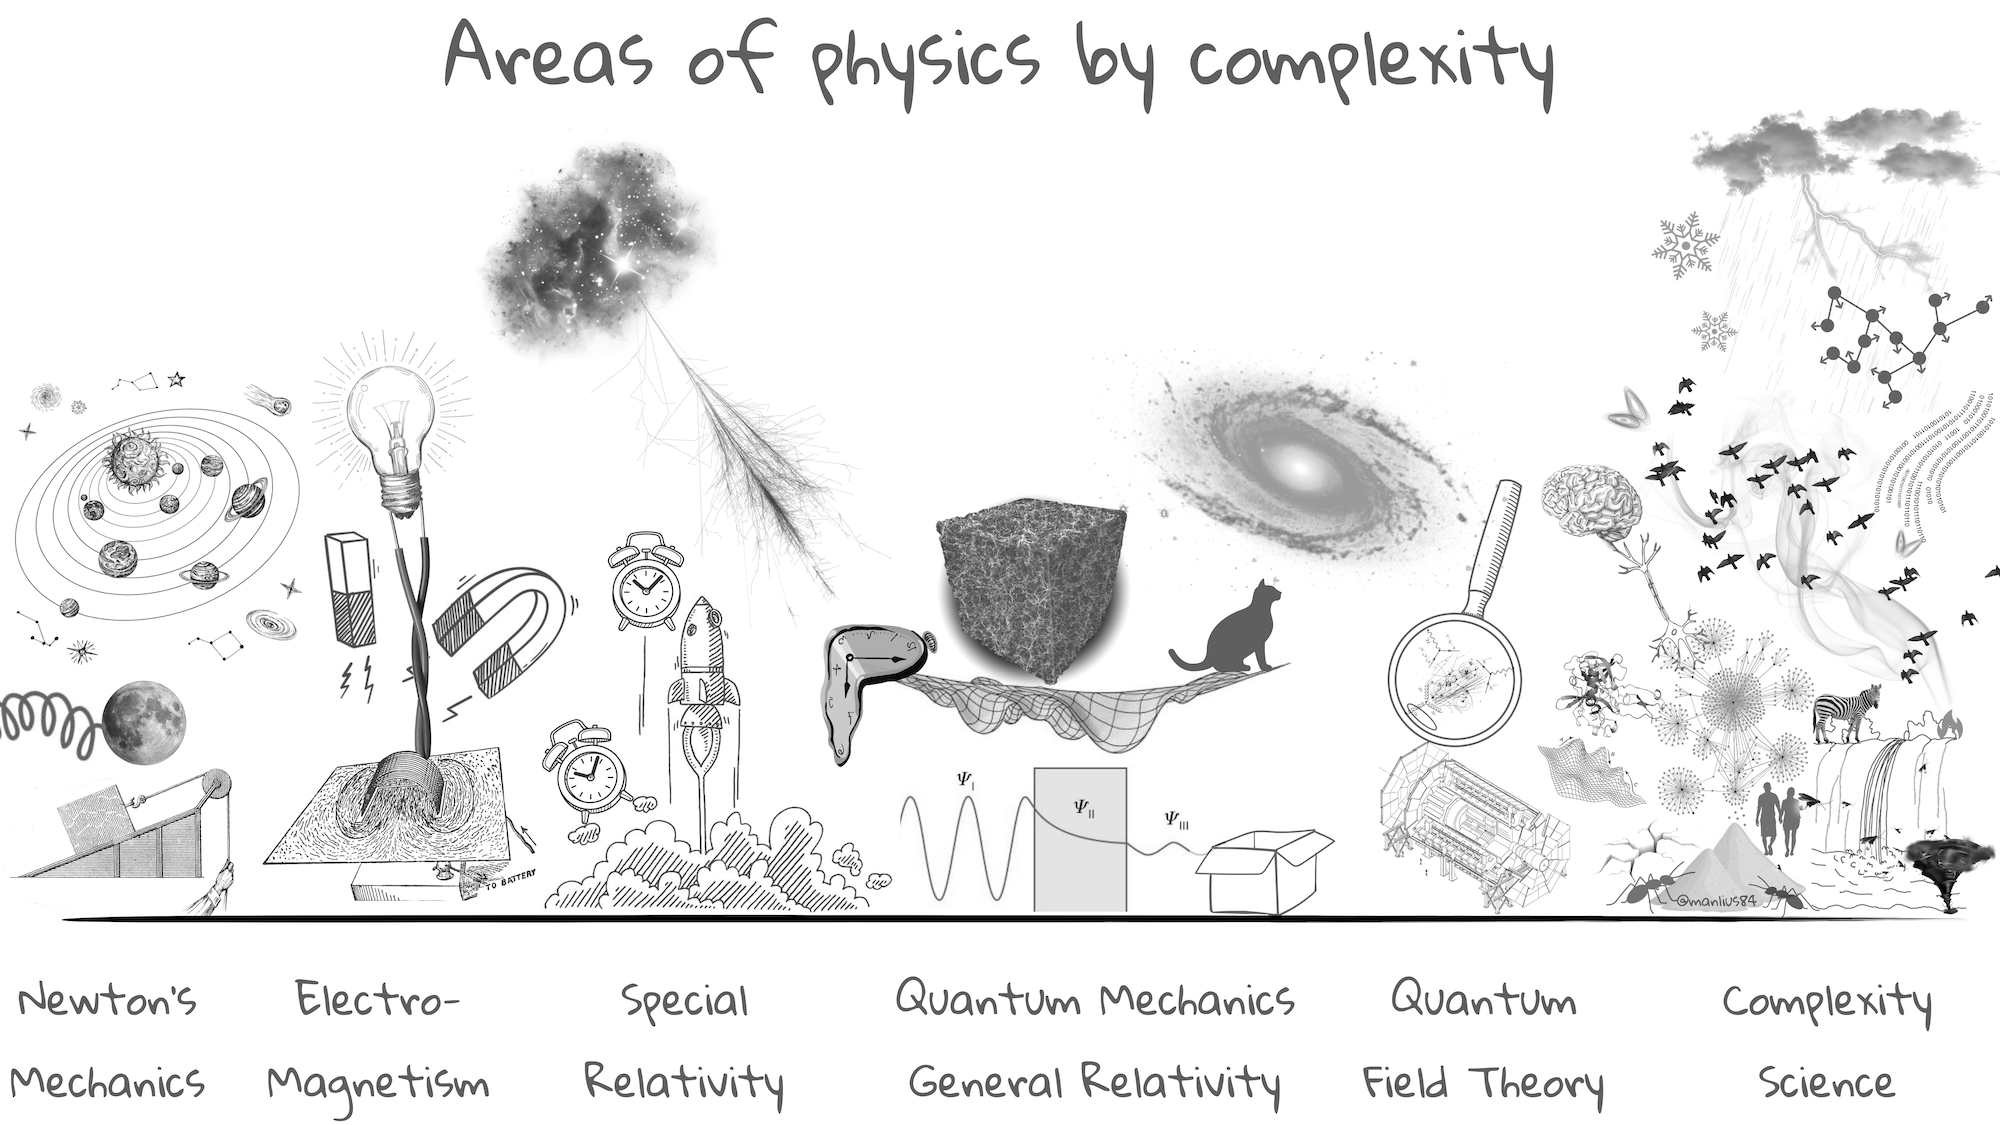
\includegraphics[width=\textwidth]{images/areas_of_physics.png} 
\end{figure}
\vspace*{1cm}
\textcolor{unipd}{\textbf{\large Physics of Complex Networks: Structure and Dynamics}} \\
\vspace*{1cm}
\textcolor{unipd}{\textbf{\huge Final Report}} \\
\vspace*{2cm}
\textbf{Student:} Zara Miriam \hfill \textbf{Last update}: \today\\
\end{center}



\thispagestyle{empty} % Prevents page number from being included on the cover
\clearpage\setcounter{page}{1} % Start including page numbers from here
\pagenumbering{roman} % in roman numerals
    
    % Index of the document and figures
    \begingroup
        % Links are normally blue, but indexes are set to black
        % so that everything does not appear blue
        \hypersetup{linkcolor=black}
        \tableofcontents
        %\listoffigures % uncomment to display list of code 
        %\lstlistoflistings % uncomment to display list of code 
        %\listof{example}{Lista degli esempi}
        %check https://tex.stackexchange.com/questions/16494/generating-lists-of-custom-environment
    \endgroup
       %Change page number style to normal
       \clearpage\pagenumbering{arabic}
    
% Sections and chapters
\titleformat{\section}[hang]{\large\bfseries}{\textcolor{unipd}{\thesection}\hsp\textcolor{gray75}{|}\hsp}{0pt}{\large\bfseries\textcolor{gray25}}[\color{unipd}{\titlerule[1.0pt]}]
% Subsection
\titleformat{\subsection}[hang]{\large\bfseries}{\textcolor{unipd}{\thesubsection}\hsp\textcolor{gray75}{|}\hsp}{0pt}{\large\bfseries\textcolor{gray25}}[\color{unipd}{}]

\chapter{Task 18: Turing Patterns}

\section{Task Description}
The goal of this task is to analyze a Turing activator-inhibitor dynamics on networks, with specific suggestion to replicate the findings of \cite{main_network}. 
\noindent
A system governed by a reaction-diffusion mechanism can exibit pattern emergence when perturbed from an initial linearly stable equilibrium state. The conditions for pattern initiation are found through linear stability analysis. The subsequent evolution of the pattern is non-linear and eventually results in a steady state (that can be either stationary or time dependent).
\\
\textbf{A note:} The authors of \cite{main_network} only state the conditions that must hold for pattern formation on the network. In fact, they can be derived with only a few minor changes in the same way as one does for pattern formation in a continuous medium. However, if the reader is not familiar with the traditional Turing patterns in continuous space (like me before this work), those relations are not at all evident. I wanted to get a true understanding of what I was going to simulate. That is why I studied in detail the case of the continuous medium and then I derived the conditions stated by the authors of \cite{main_network}. However, this meant that, to keep the workload manageable, I was able to focus only on the analysis of the \textbf{pattern initiation} stage and disregard the anaylis of the multistability and histeresis effects done in the second part of the article.

\section{Mathematical Model}
\subsection{Definitions}
A network-organized activator-inhibitor system can be defined in very close analogy to what one does for continuous media. 
In the network case, equations for the system are:
$$
\begin{cases}
\dot{u}_i(t) = f(u_i\, v_i) - \epsilon\,[L\,u(t)]_i \\
\dot{v}_i(t) = g(u_i\, v_i) - \epsilon\, \sigma [L\,v(t)]_i \\
\end{cases}
$$
Here, $\mathbf{u} = (u_1, \cdots u_N)$ and $\mathbf{v} = (v_1, \cdots v_N)$ are, respectively, the concentrations of the activator substance and the inhibitor substance on the $N$ nodes of the network. The reactions take place locally, on each node, and are encoded in the reaction terms $f(u_i\, v_i)$ and $f(u_i\, v_i)$. L is the laplacian matrix, defined as $L=D-A$. The diffusivity of the activator species is $\epsilon$, while that of the inhibitor is $\epsilon\,\sigma$, so that $\sigma$ is the ratio between them.

So far, the above are just the general equations of a reaction-diffusion system. In order to have a Turing mechanism, the reaction term need to satisfy the following basic requirements:
\begin{enumerate}
	\item Existence of a homogeneous equilibrium $(\overline{u},\, \overline{v})$ which is linearly stable in absence of diffusion (indeed, the key idea of the Turing model is that the instability is driven by diffusion, and appears only above a certain threshold function of the diffusion parameters) :
		$$
		\centering
		\begin{pmatrix}
			u_i(t) \\
			v_i(t)
		\end{pmatrix} \equiv  
		\begin{pmatrix}
			\overline{u} \\
			\overline{v}
		\end{pmatrix}
        \quad \forall i 
		\quad \text{where} \quad f(\overline{u}\,, \overline{v}) = g(\overline{u}\,, \overline{v})=0 \quad \text{and, given that}
		$$
		$$
		 \quad J(\overline{u}\,, \overline{v}) := 
		\begin{pmatrix}
 			f_u & f_v \\
 			g_u & g_v
 		\end{pmatrix}, \quad
 		\begin{cases}
 			\text{tr}(J)= f_u + g_v < 0\\
 			\text{det}(J) = f_u\cdot g_v f_v\cdot g_u>0
 		\end{cases}
		\text{(see \ref{app:bifurcation_diagram})}
		$$
	\item Correct qualitative behaviour of reactions in the neighborhood of the fixed point $(\overline{u},\, \overline{v})$: \newline
    the activator $u$ is supposed to enhance its own production and the production of the inhibitor $v$. Viceversa, the inhibitor $v$ is supposed to suppress the production of both the activator $u$ and itself. The functions $f,\, v$ need to reflect this behaviour, at least in a neighbourhood of the equilibrium $(\overline{u},\, \overline{v})$. Mathematically:
    \begin{center}
    \begin{minipage}{0.4\textwidth}
    \centering
    $$
           \begin{cases}
         f_u > 0,\quad f_v < 0 \\
         g_u >0,\quad  g_v <0 \\      
        \end{cases} 
    $$
    \end{minipage}
    \begin{minipage}{0.5 \textwidth}
    \centering
	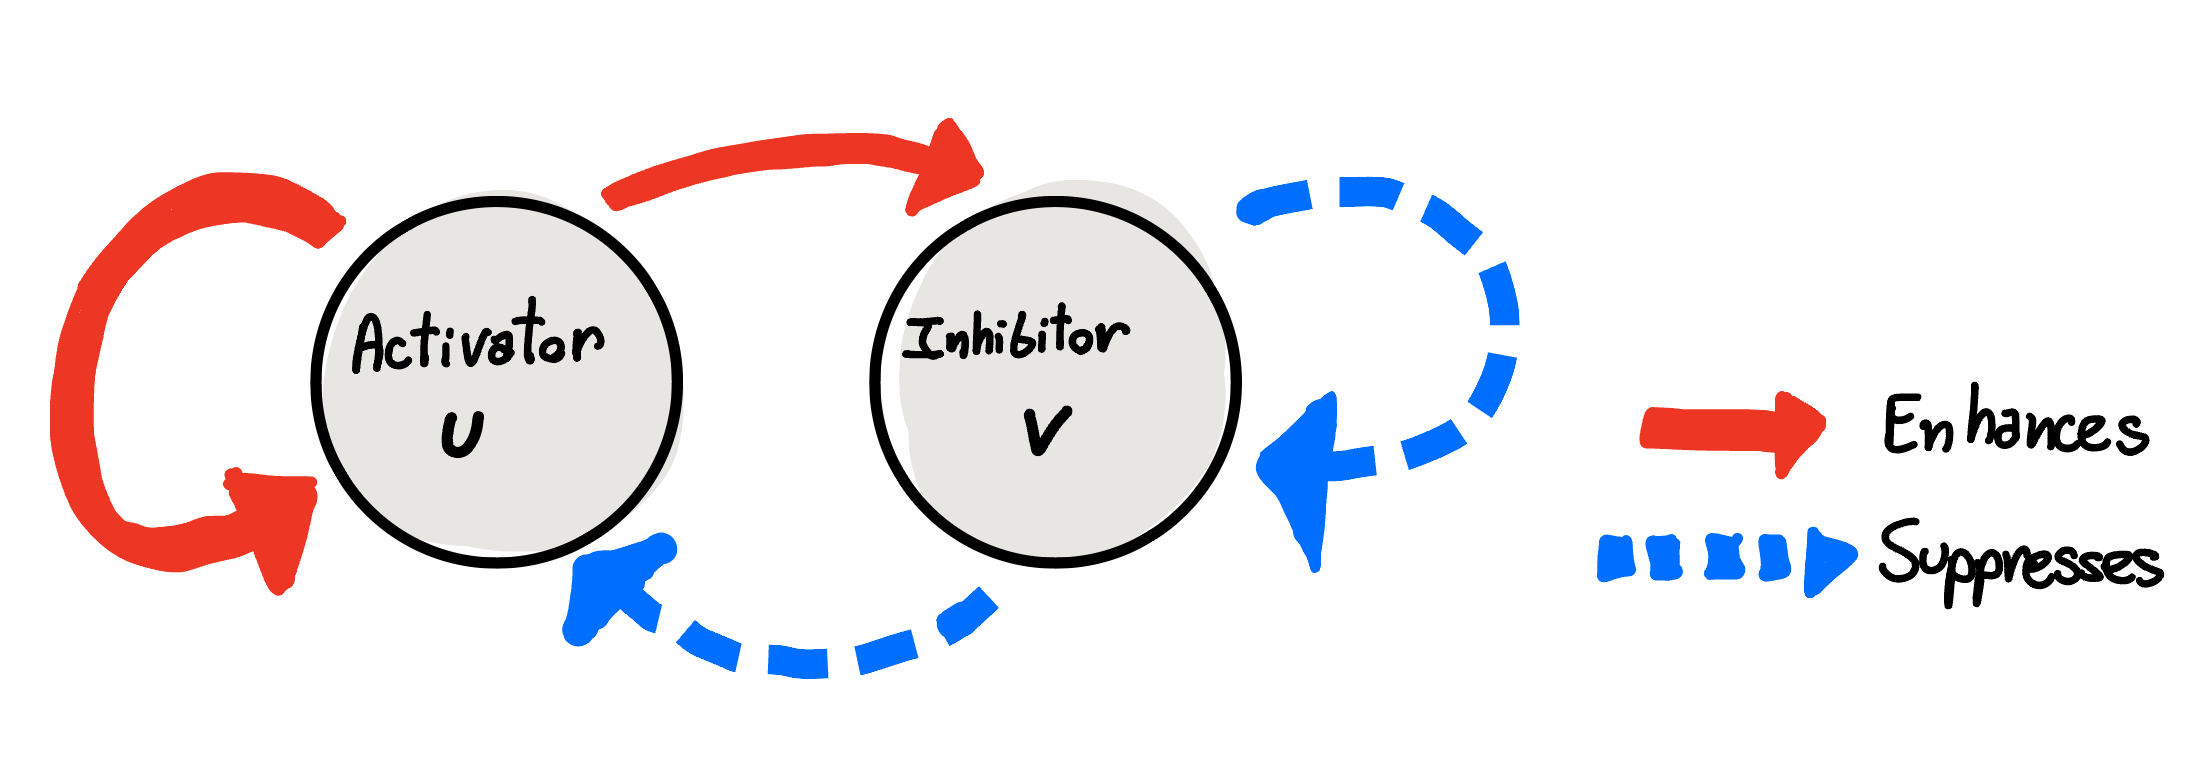
\includegraphics[width=0.9\textwidth]{images/turing/diagram.jpeg}
 \label{fig:diagram}
    \end{minipage}
    \end{center}
\end{enumerate}
These requirements are just the same as in the case for the continuous medium. 
\subsection{Conditions for diffusion-driven instability}
Diffusion driven instability is investigated by means of linear stability analysis. A small random perturbation $\delta\,u_i,\, \delta\,v_i$ is added at each node, starting from the homogeneous equilibrium state. A linearized system of equations is obtained for the evolution of the perturbation:
\begin{equation}
    \begin{cases}
    u_i(t) = \overline{u} + \delta\, u_i(t)\\
    v_i(t) = \overline{v} + \delta\, v_i(t)
    \end{cases}
    \rightarrow 
    \begin{cases}
    \delta\, \dot{u}_i(t) \simeq \quad     f_u\, \delta u_i(t) +  f_v\, \delta v_i(t) - \epsilon\,[L\cdot (\overline{u}+ \delta u(t))]_i\\
    \delta\, \dot{v}_i(t) \simeq \quad 
    g_u \, \delta u_i(t) +  g_v \, \delta v_i(t) - \epsilon\,\sigma\,[L(\overline{v}+ \delta v(t))]_i
    \end{cases}
\end{equation}
But $L\,\overline{u} = L\,\overline{v} = 0$, since the constant vectors $u$ and $v$ are eigenvectors of the laplacian with eigenvalue zero.
In the case of a continuous medium, the perturbation is expanded as a Fourier series of plane waves. The rationale of this is that it makes the PDE turn into an eigenvalue problem.
In the network case, we instead write the perturbation as:
\begin{equation*}
    \begin{pmatrix}
    \delta u_i (t) \\
    \delta v_i (t) \\
    \end{pmatrix}
    =
    \begin{pmatrix}
        1 \\
        B_n \\
    \end{pmatrix}
    \cdot \sum_{n=1}^{N}\, c_n\,\Phi_i^{(n)}\, e^{\lambda_n\,t} \\
\end{equation*}
Where $\Phi^{(n)}$ is the $n-th$ eigenvector of the laplacian matrix $L$ and its corresponding eigenvalue is $\Lambda_n$ ($0=\Lambda_1 \leq \Lambda_2 \leq \cdots \Lambda_N$). The coefficients $\{c_n\}$ are determined by the initial conditions $(t=0)$. By doing this, the system of equations is turned into a $\Lambda -$dependent eigenvalue problem. In fact, if we plug the ansaltz 
\begin{equation*}
    \begin{pmatrix}
    \delta u_i (t) \\
    \delta v_i (t) \\
    \end{pmatrix}
    =
    \begin{pmatrix}
        1 \\
        B_n \\
    \end{pmatrix}
    \cdot  c_n\,\Phi_i^{(n)}\, e^{\lambda_n\,t} \\
\end{equation*}
into the linearized system of equations, we get:
\begin{equation*}
    \begin{pmatrix}
        \delta \dot{u}_i \\
        \delta \dot{v}_i \\
    \end{pmatrix}
    =
    \begin{pmatrix}
        f_u - \epsilon\,\Lambda_n & f_v \\
        g_u & g_v -\epsilon\,\sigma\,\Lambda_n \\
    \end{pmatrix}
    \cdot 
        \begin{pmatrix}
        \delta u_i \\
        \delta v_i \\
    \end{pmatrix}
\end{equation*}
\begin{equation*}
    \rightarrow
        \lambda_n \cdot
        \begin{pmatrix}
        1 \\
        B_n\\
    \end{pmatrix}
    =
    \begin{pmatrix}
        f_u - \epsilon\,\Lambda_n & f_v \\
        g_u & g_v -\epsilon\,\sigma\,\Lambda_n \\
    \end{pmatrix}
    \cdot 
        \begin{pmatrix}
        1 \\
        B_n\\
    \end{pmatrix}
\end{equation*}
Or, in compact form:
\begin{equation*}
    \lambda_n\, \mathbf{v}_n = M(\Lambda_n,\,\sigma,\,\epsilon)\, \mathbf{v}_n
\end{equation*}
The differences between the network case and the continuous medium case end here. From now on, the steps are exactly the same. We are looking for instability, thus we want to find the range of parameters $(\sigma,\, \epsilon)$ that produce $\mathcal{R}e\{\lambda_{\pm}(\Lambda)\}>0$ for a positive range of $\Lambda$'s. \\
First, we must have that at least one of the following holds
\begin{equation*}
    \begin{cases}
        \text{det}[M(\Lambda,\,\sigma,\,\epsilon)]<0 \\
        \text{tr}[M(\Lambda,\,\sigma,\,\epsilon)]> 0 \\
    \end{cases}
\end{equation*}
But $\text{tr}[M(\Lambda,\,\sigma,\,\epsilon)] = \text{tr}[J] - \epsilon\, \Lambda\, (1+\sigma)<0$ because the homogeneous state is a stable equilibrium, then the only possibility is that $\text{det}[M(\Lambda,\,\sigma,\,\epsilon)]< 0$. \\
Some quick boring algebra now:
\begin{equation*}
    \text{det}[M(\Lambda,\,\sigma,\,\epsilon)] = \epsilon^2\,\sigma\,\Lambda^4 - \epsilon\,(g_v +\sigma\,f_u) \Lambda + \text{det}[J] \overset{!}{\leq} 0 \quad \text{for some}\, \Lambda >0
\end{equation*}
\begin{minipage}{0.6\textwidth}
This is a parable of kind $y = a\,x^2 - b\,x + c$ with  $(a,\,b,\,c>0)$, so the minimum is reached at coordinates $(x_{min},\,y_{min}) = (\frac{b}{2\,a}\,, c-\frac{b^2}{4\,a})$. The parable touches the $x$ axis ($y_{min}\leq 0$) $\iff$ $\Delta^2 = b^2-4\,a\,c \geq 0$.
\end{minipage}
\hfill
\begin{minipage}{0.38\textwidth}
    \centering
    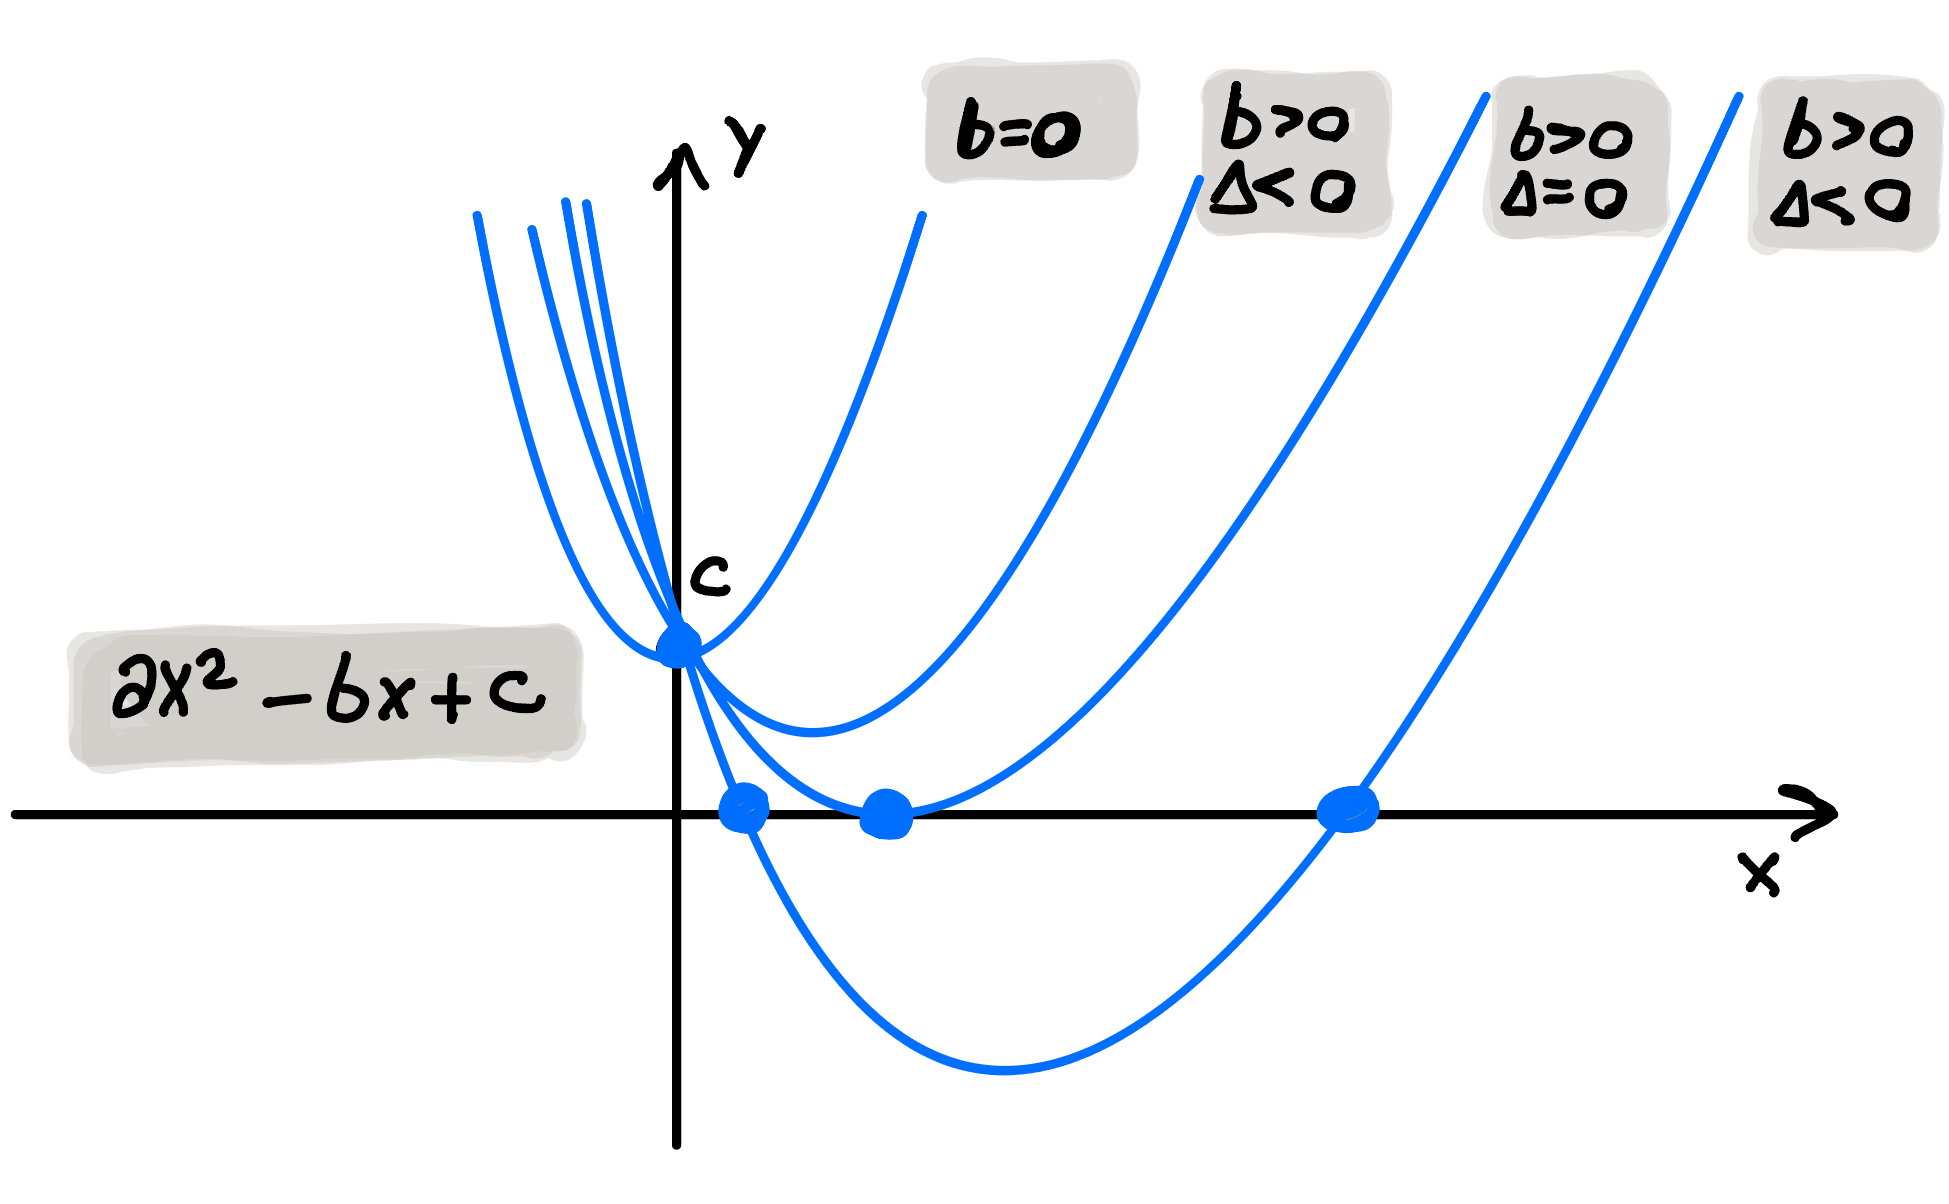
\includegraphics[width=\textwidth]{latex_source/images/turing/parable.jpeg}
\end{minipage}
\newline
We require:
\begin{equation*}
    \begin{cases}
        x_{min}(\epsilon,\,\sigma)>0 \\
        y_{min}(\epsilon,\,\sigma)\leq 0 \\
    \end{cases}
    \quad
        \begin{cases}
        \epsilon\,(g_v +\sigma\,f_u) > 0 \\
        [\epsilon\,(g_v +\sigma\,f_u)]^2 \geq 4\,\epsilon^2\,\sigma\,\text{det}[J] \\
    \end{cases}
\end{equation*} 
\begin{figure}[H]
    \centering
    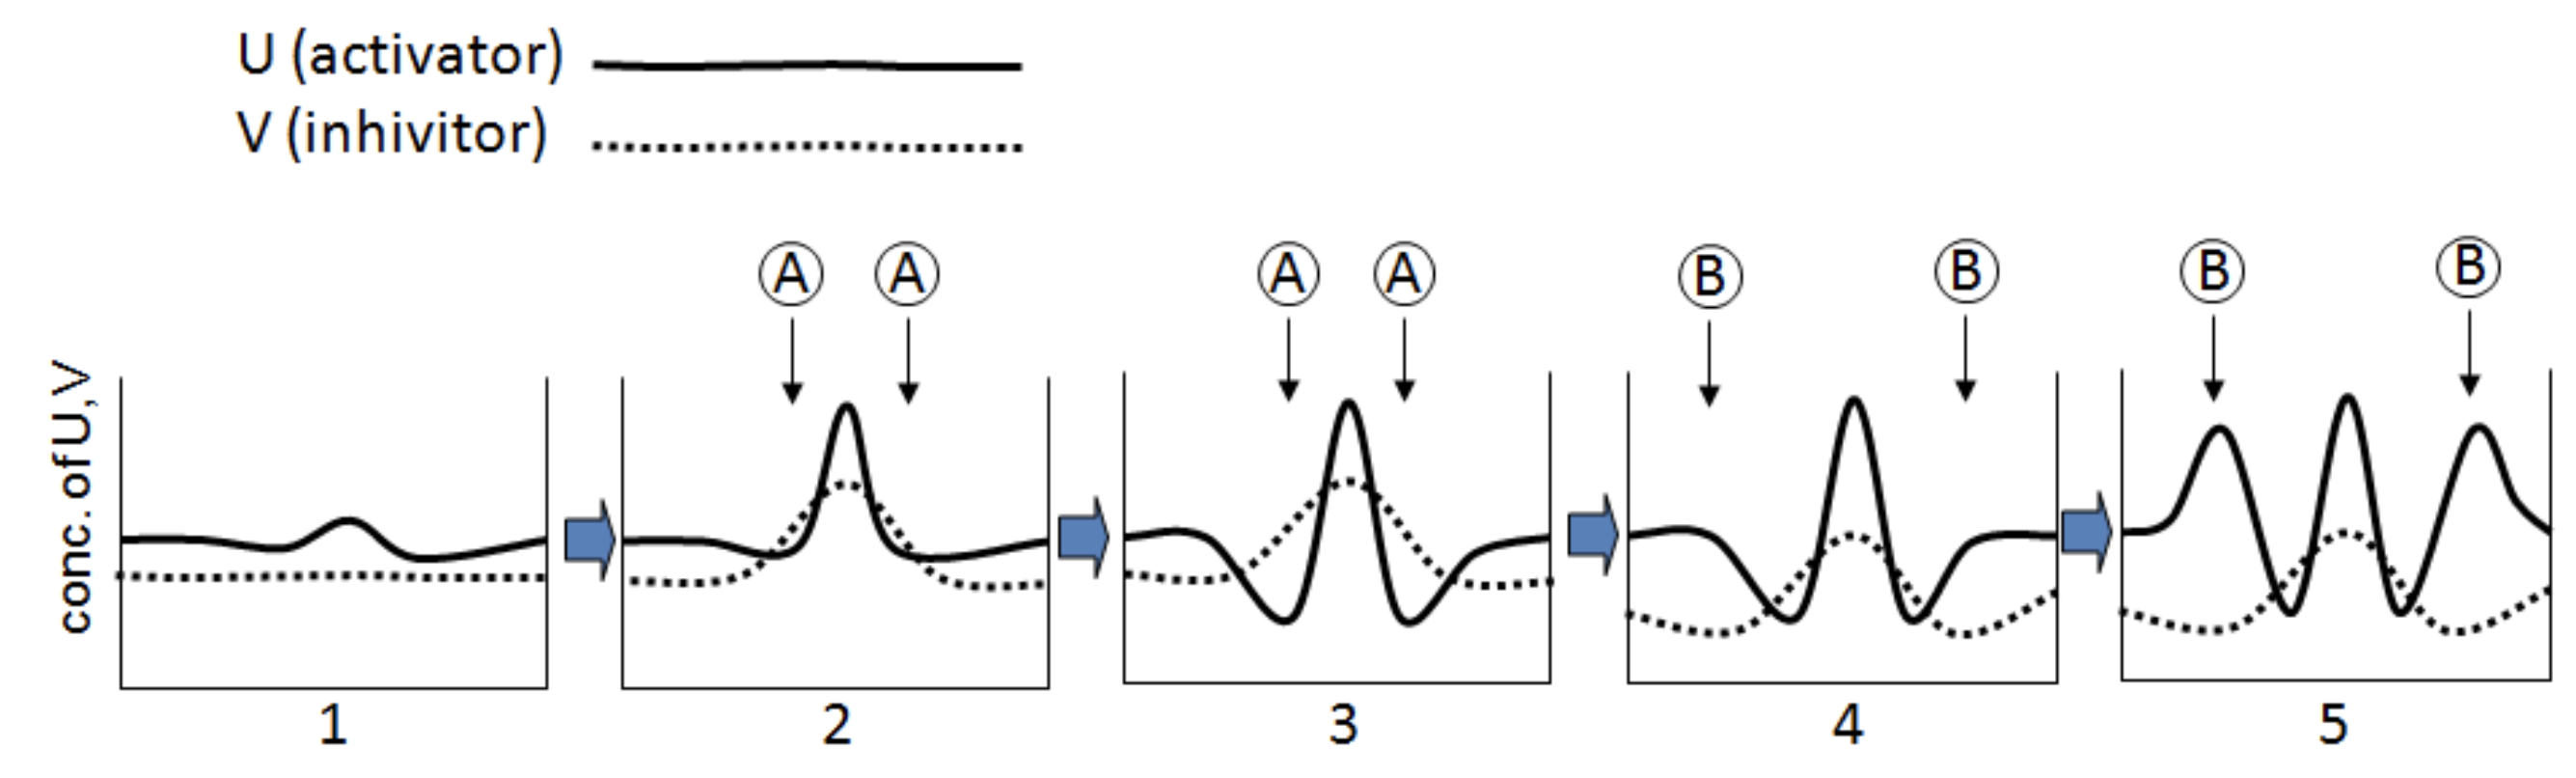
\includegraphics[width=\linewidth]{latex_source/images/turing/key_mechanism.png}
    \label{fig:key}
    \caption{{\small Graph 1 shows the initial condition of the system. Suppose that the concentration of the
activator is relatively higher than in other regions by random fluctuation. By the
self-enhancing property of the activator, the concentration of activator increases at the
center region (graph2), followed by the increase of inhibitor at the neighboring region A.
As the diffusion rate of inhibitor is much larger than that of the activator, substantial
amounts of inhibitor move toward the lateral regions. This depresses the activator
function, resulting in the decrease of the activator concentration there (graph3).
Decrease of activator causes the decrease of inhibitor in the wider region (graph4). At
the region B, as inhibitor concentration is gotten lower, activator becomes relatively
dominant than inhibitor. This situation is enough to start the local self activation at
region B (graph5). \parencite[Figure taken from][Supplementary Information]{bio_article}. }}
   \label{fig:key}
\end{figure}
\noindent 
From the first one, we notice that there exists a minimum value threshold for $\sigma > \sigma_{min}= \frac{|g_v|}{f_u}$. Also, since $\text{tr}\,[J]=(-|g_v| +f_u)<0$, then $\sigma_{min}> 1$: a necessary (but still not sufficient) condition for pattern initiation is that the inhibitor diffuses faster than the activator. Indeed, this difference between the diffusion constants of the two species is key to have patterns induced by diffusion (see Figure \ref{fig:key}.)
\begin{equation*}
    \begin{cases}
        \sigma > \sigma_{min} >1  \\
        f_u^2\,\sigma^2 + 2\,(f_u\,g_v-2\,\text{det}[J])\,\sigma + g_v^2 \geq 0 
    \end{cases}
    \quad 
    \begin{cases}
    \sigma > \sigma_{min} >1  \\
    \sigma < \sigma_{-}(<\sigma_{min}) \quad \text{or} \quad  \sigma > \sigma_{+}\\
    \end{cases}
\end{equation*} 
Where $\sigma_{\pm}$ are the roots of the quadratic equation:
\begin{equation*}
    \sigma_{\pm} = \frac{(f_u\,g_v - 2\,f_v\,g_u)\,\pm 2\,\sqrt{f_v\,g_u\,(f_v\,g_u-f_u\,g_v))}}{f_u^2}
\end{equation*}
The function $y_{min}(\sigma)$ reaches its maximum for $\sigma=\sigma_{min}$ and goes to $-\infty$ for both $\sigma\rightarrow0^{+}$ and $\sigma\rightarrow +\infty$. Also, the lower-branch root $\sigma_{-}$ is below the threshold value $\sigma_{min}$. Then, both our requirements are satisfied if and only if $\sigma>\sigma_{+}$. In summary, the necessary and sufficient condition for instability is
\begin{equation*}
 \sigma > \sigma_c :=  \frac{(f_u\,g_v - 2\,f_v\,g_u)\, + 2\,\sqrt{f_v\,g_u\,(f_v\,g_u-f_u\,g_v))}}{f_u^2}
\end{equation*}
\textbf{Critical eigenvalue and graph finite size effect} \newline
The critical eigenvalue $\Lambda$ is determined for give $\epsilon$:
\begin{equation}
\label{eq:critical_eigenvalue}
    \Lambda_c(\epsilon) := \Lambda(\sigma=\sigma_c,\,\epsilon) = \frac{g_v + \sigma_c\,f_u}{2\,\epsilon \,\sigma_c} = (\cdots) = \frac{1}{\epsilon}\,\sqrt{\frac{\text{det}[J]}{\sigma_c}}
\end{equation}
For $\sigma$ above the critical threshold, a finite range [$\Lambda_1\,\Lambda_2$] centered around $\Lambda_c$ appears where the corresponding mode is unstable. However, the eigenvalue spectrum of the laplacian matrix is not continuous. Instability will appear if there are allowed modes that fall inside this range.
In particular, the eigenvalue spectrum of the laplacian is bounded above for a graph of finite size. If the mobility $\epsilon$ is small enough, the critical eigenvalue could lay beyond the largest eigenvalue of the graph, and instability would not occur.
This finite-size effect appears also in the case of a continuous medium. There, instability cannot occur when the spatial domain is too small and the largest allowed wavelength is less than the critical wavelength.
\medskip \newline
\textbf{Dispersion relation $\lambda(\Lambda;\, \sigma,\,\epsilon)$} \newline
Finally, the growing rate of the unstable mode, $\lambda_n = \lambda(\Lambda_n)$ is calculated from the caractheristic polynomial of $M(\Lambda_n, \sigma,\,\epsilon)$:
\begin{equation*}
    p(\lambda) = (\lambda-\lambda_1)\cdot(\lambda-\lambda_2) = \lambda^2 - \text{tr}[M(\Lambda,\,\sigma,\,\epsilon)]\cdot \lambda + \text{det}[M(\Lambda,\,\sigma,\,\epsilon)]
\end{equation*}
\begin{align*}
    \lambda_{\pm} &=\frac{1}{2}\,\left[\text{tr}[M]\pm \sqrt{\text{tr}[M]^2-4\,\text{det}[M]}\right] = \frac{1}{2}\,\left[-|\text{tr}[M]|\pm \sqrt{\text{tr}[M]^2-4\,\text{det}[M]}\right] \\
    &= \frac{1}{2}\, \left[\left[f_u + g_v - (1+\sigma)\,\epsilon\,\Lambda\right] + \sqrt{4\,f_v\,g_u + \left[f_u - g_v -(1-\sigma)\,\epsilon\,\Lambda\right]^2}\right]
\end{align*}
In the instability region, $\text{tr}[M] <0$ and $\text{det}[M]<0$, then eigenvalues are real and distinct. Also, the lower branch is always negative so we are not interested in it. By comparison with the graph of $\text{det}[M(\Lambda,\,;\epsilon,\,\sigma]$, we get the qualitative dependence of $\lambda$ from $\Lambda$, commonly called "dispersion relation".
\newpage
\section{Numerical Simulations}
As in \cite{main_network}, the reaction terms are set as
\begin{equation}
    \begin{cases}
        f(u,v) = [\frac{a + b\,u -u^2}{c} - v]\, u \\
        g(u, v) = [u - (1+ d\,v)]\cdot v 
    \end{cases}
\label{eq:chosen_kinetics}
\end{equation}
with parameters $a\,=\,35,\, b=16,\, c= 9,\, d= 2/5$, 
helding a linearly stable fixed point $(\overline{u},\, \overline{v}) = (5, 10)$ and a critical diffusion ratio $\sigma_c \simeq 15.5$. \newline \noindent
\begin{figure}[H]
    \centering
    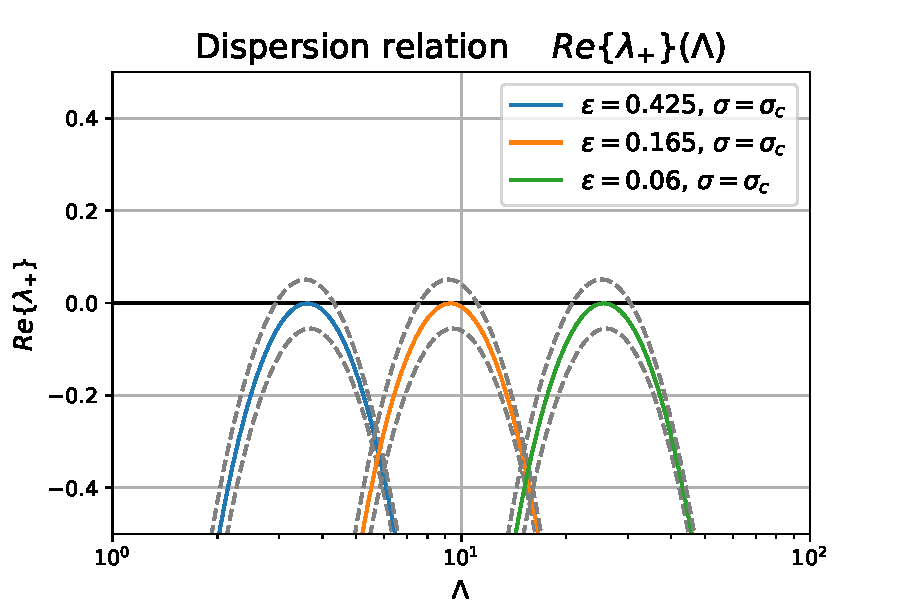
\includegraphics[width=0.8\textwidth]{latex_source/images/turing/multiple_dispersion.pdf}
    \caption{Dispersion relation for the chosen reaction kinetics [Eq. $\ref{eq:chosen_kinetics}$], at different values of the activator diffusivity $\epsilon$. The dashed grey lines are the dispersion curves slightly above and below the critical diffusivity ratio $\sigma_c$. As stated in [Eq. \ref{eq:critical_eigenvalue}], the critical eigenvalue $\Lambda_c$ is inversely proportional to the activator diffusivity $\epsilon$.}
\end{figure}
Following the choice of the authors, I simulated the dynamics on Barabasi-Albert scale free networks. I chose parameters $N = 200$ for the number of nodes and $\<k\> = 10$ for the mean degree. My activator diffusivity was $\epsilon = 0.12$, and my diffusivity ratio was $\sigma = 15.6 > \sigma_c = 15.5$. The reasoning for chosing a diffusivity ratio that is only slightly above the critical threshold is to keep the number of different allowed modes low.
\begin{figure}[H]
\subfigure[]{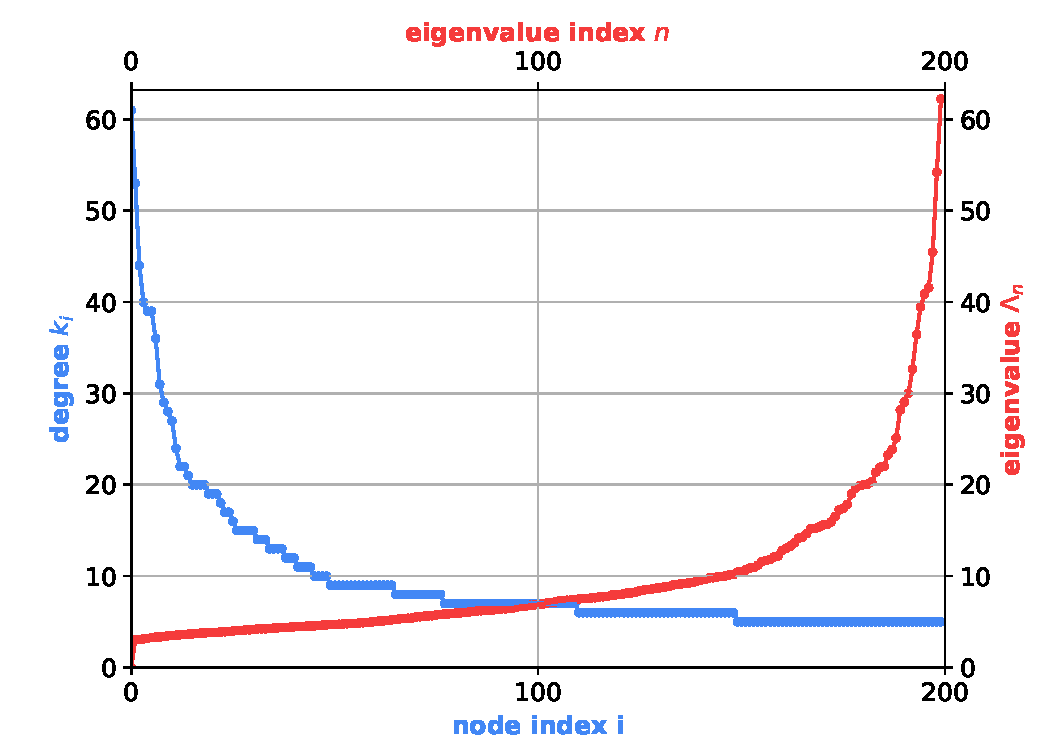
\includegraphics[width = 0.47\textwidth]{latex_source/images/turing/network_200.pdf}}
\subfigure[]{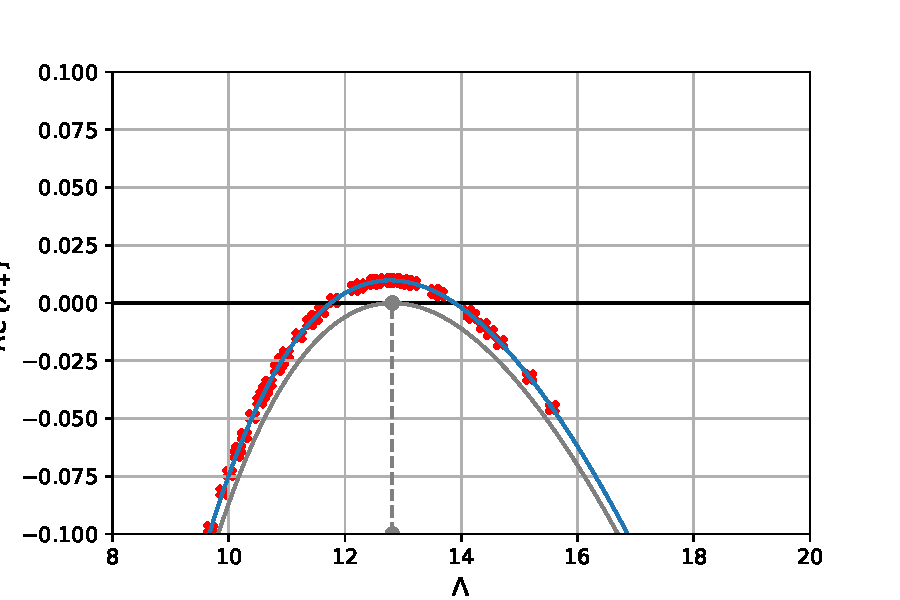
\includegraphics[width = 0.47\textwidth]{latex_source/images/turing/simulation_dispersion.pdf}}
\caption{Most relevant properties of the network used in the simulation. Subfigure (a) shows the degree spectrum and the laplacian eigenvalue spectrum of the chosen graph. Network nodes are indexed by decreasing degree. Subfigure (b) shows the dispersion relation curve. Critical eigenvalue is $\Lambda_c \simeq 12.8141$. The eigenvalue closest to $\Lambda_c$ is $\Lambda_n \simeq 12.64$, of index $n=157$. However, as one can see from the graph, the network eigenvalue spectrum comprehends several other allowed modes (red crosses) in the unstable range, and they are expected to contribute to pattern initiation as well.}
\end{figure}
\noindent
The initial homogeneous state $(\overline{u},\,\overline{v})$ was perturbed with a random uniform perturbation at each node of amplitude $0.05$. [Figure \ref{fig:snapshots}] show snapshots of the activator concentration on nodes at different times. Also, the GithHub repository \cite{git} contains a .mp4 video of the whole evolution. \medskip \newline \noindent
In the early stage, the pattern is expected to grow proportionally to the critical eigenvector, which is is the mode of largest growing rate: $\delta\,u(t),\, \delta\,v(t) \propto \Phi^{(n)}$.
In fact, when the initial uniform perturbation dies out and the pattern starts to grow, the activator substance distribution is located similarly to the critical eigenvector (see snapshot $t = 25.06$). Later on, the evolution becomes strongly non-linear and the pattern is reshaped (see snapshot at $t = 100.25$), till it settles into a stationary state (see snapshot at $t = 150.38$) where nodes are split into one activator-rich group and one activator-poor group. The authors found that this peculiar behaviour is well described in the framework of a mean field theory \cite{main_network}. \medskip \newline \noindent
An interesting thing one can notice in the initial stage pattern [Figure \ref{fig:snapshots}, snapshot at $t = 25.06$] is that the significant variations of the activator level are localized on a subset of nodes of close degree ($k \sim 25-75$). That is, only a specific subset of the network undergoes differentiation. This effect is was not a fortuity but is due to the fact that the laplacian eigenvectors in a large graph with a broad degree distribution tend to be localized around a specific degree $\overline{k}(\Lambda)$. Also, as authors report, a simple relation $\overline{k}(\Lambda) \simeq \Lambda$ seems to hold. I checked wether I could find the same behaviour for my graph (see [Figure \ref{fig:eigenvectors}] and [Figure \ref{fig:heatmap}].
\begin{figure}[H]
    \centering
    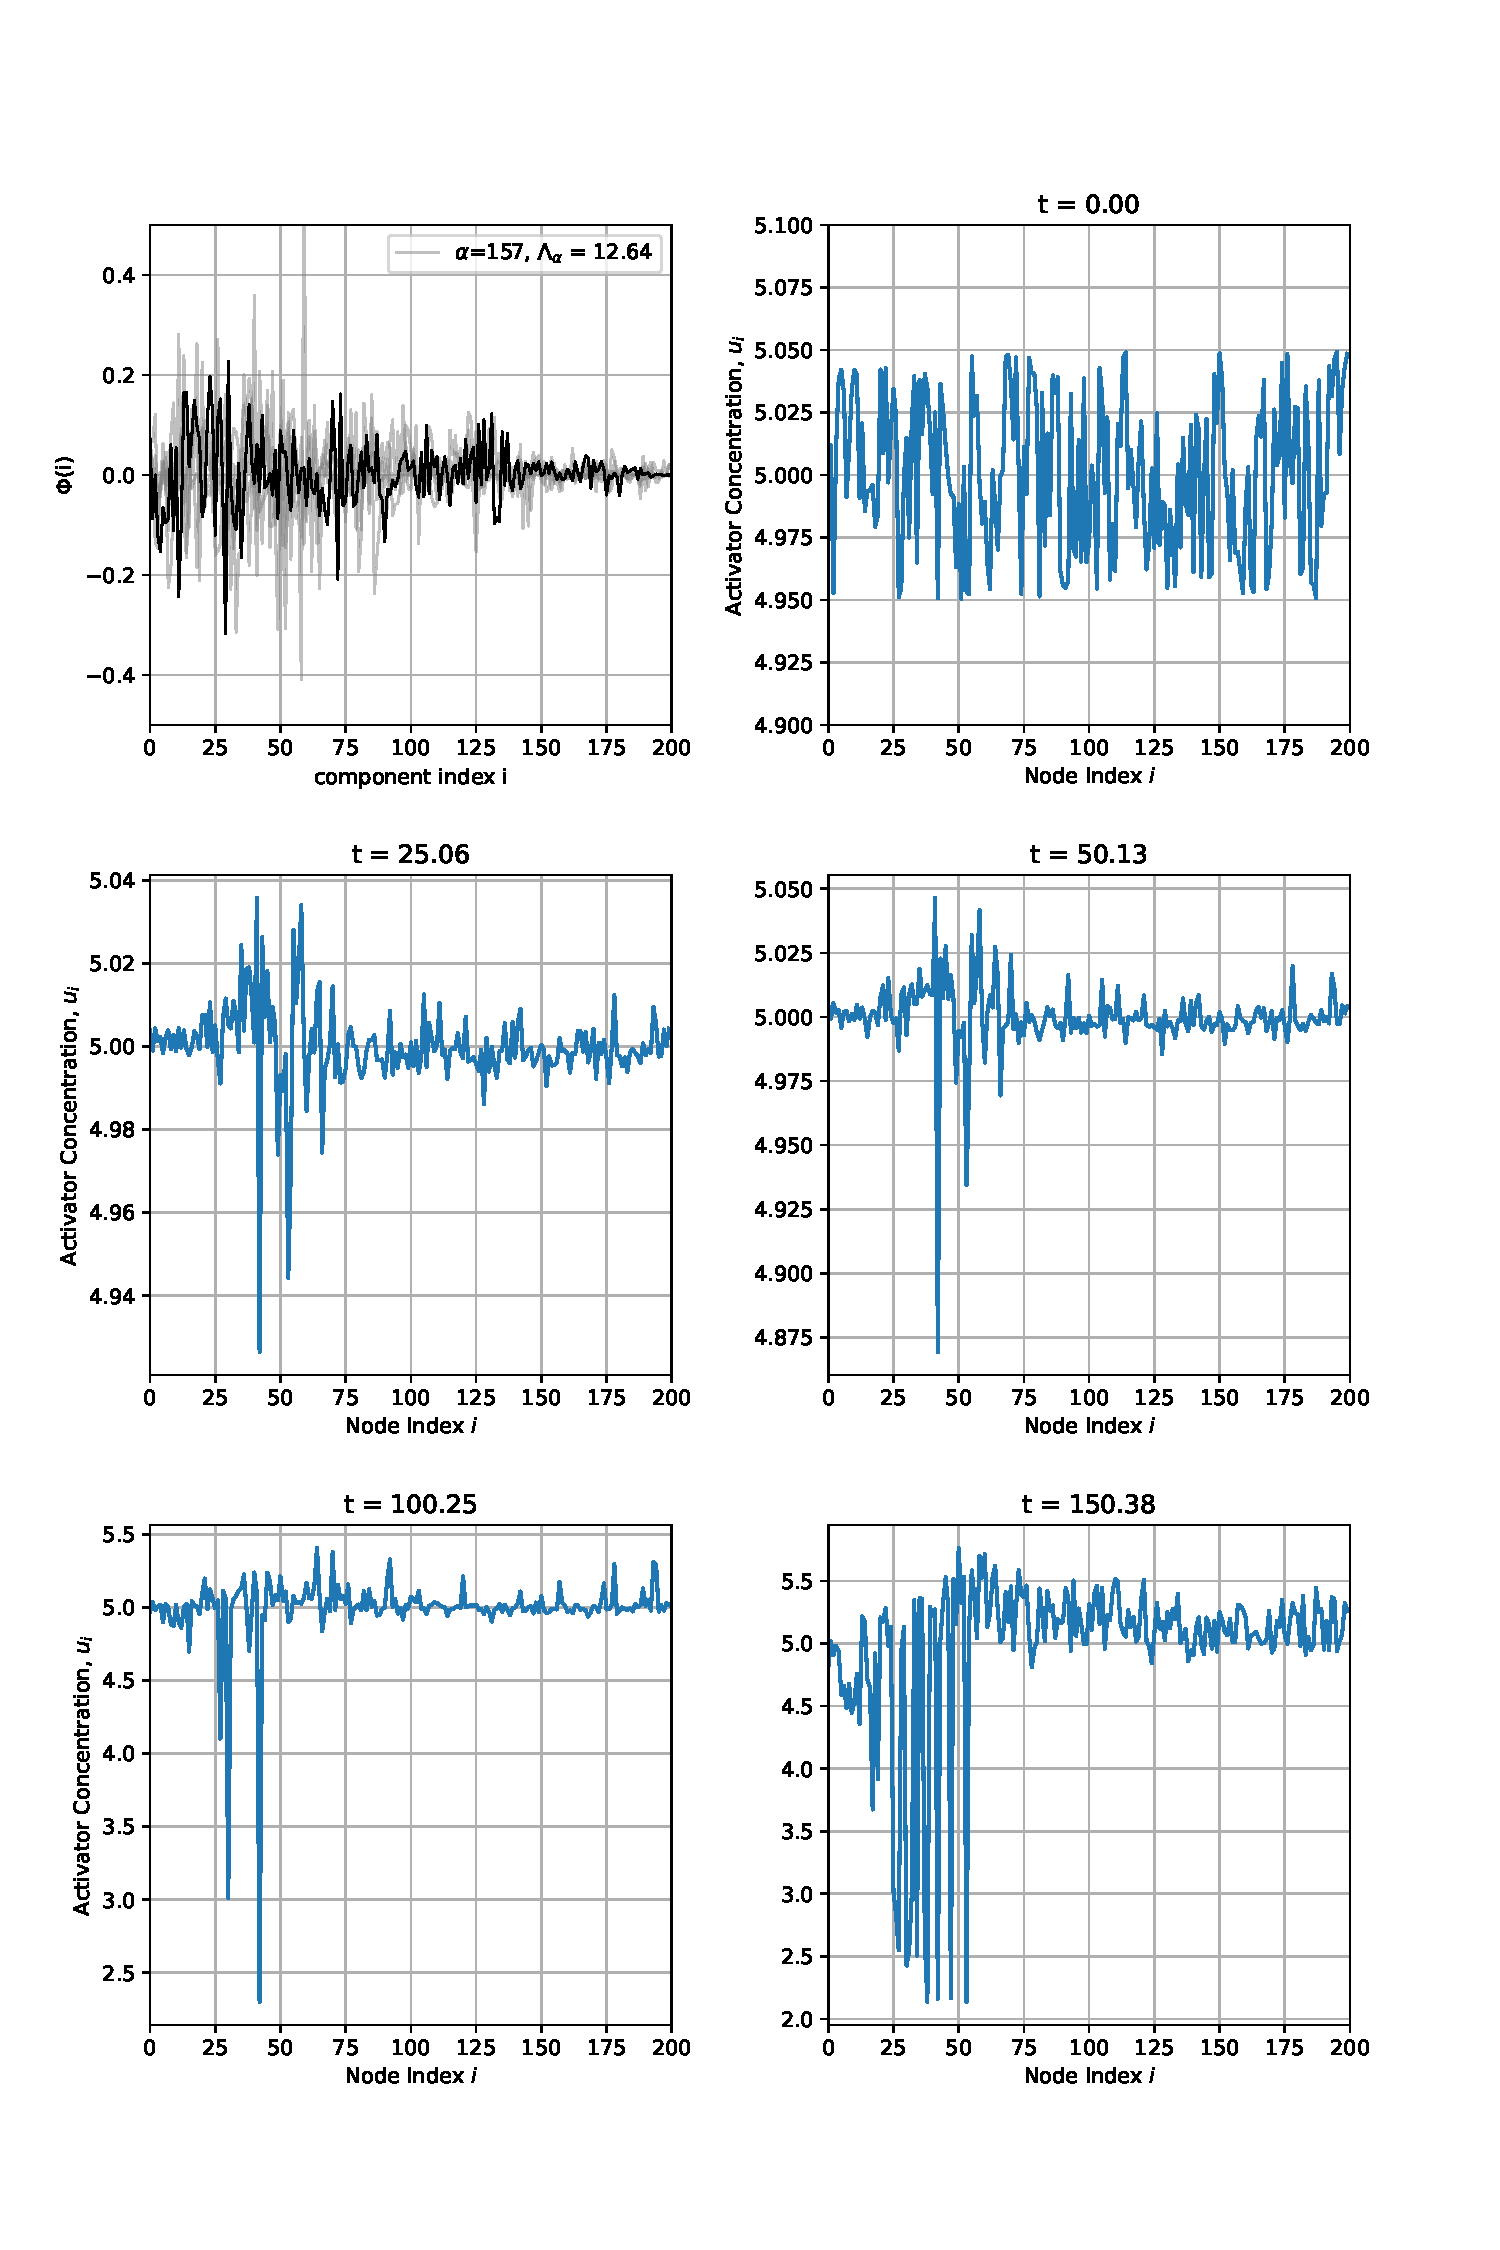
\includegraphics[width = 0.9\textwidth]{latex_source/images/turing/snapshots.pdf}
    \caption{Time evolution of the activator concentration. The subfigure at top left corner shows the components of the critical eigenvector (in black) and its closest neighbours in the unstable range (in grey).}
    \label{fig:snapshots}
\end{figure}
\begin{figure}[H]
\centering
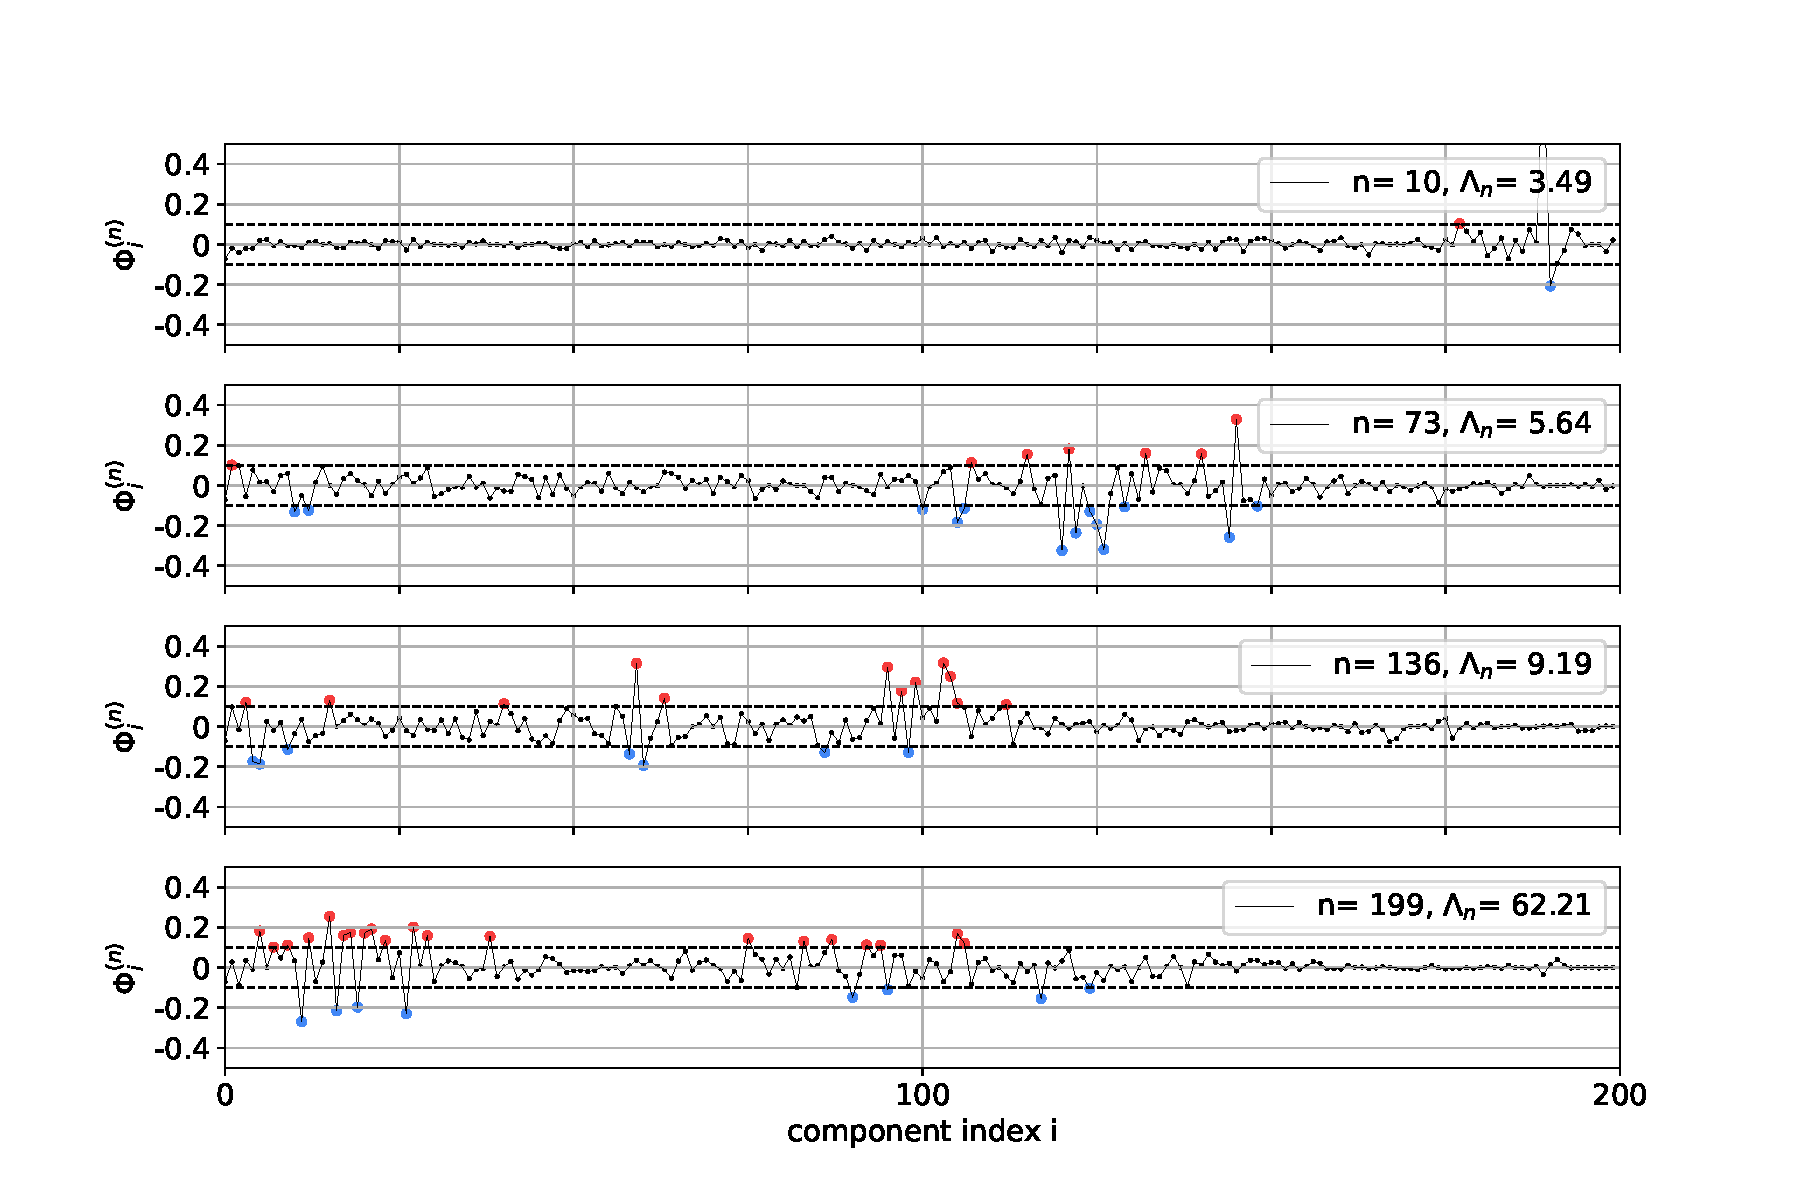
\includegraphics[width =\textwidth]{latex_source/images/turing/eigenvectors_200.pdf}
\caption{Localization of laplacian eigenvectors in 
a BA with $N=200$ and $\<k\> = 10$. Nodes nodes are ranked by their degree. With incrementing eigenvalue $\Lambda$, the characteristic degree becomes higher.}
\label{fig:eigenvectors}
\end{figure}

\begin{figure}[H]
    \centering
\subfigure[]{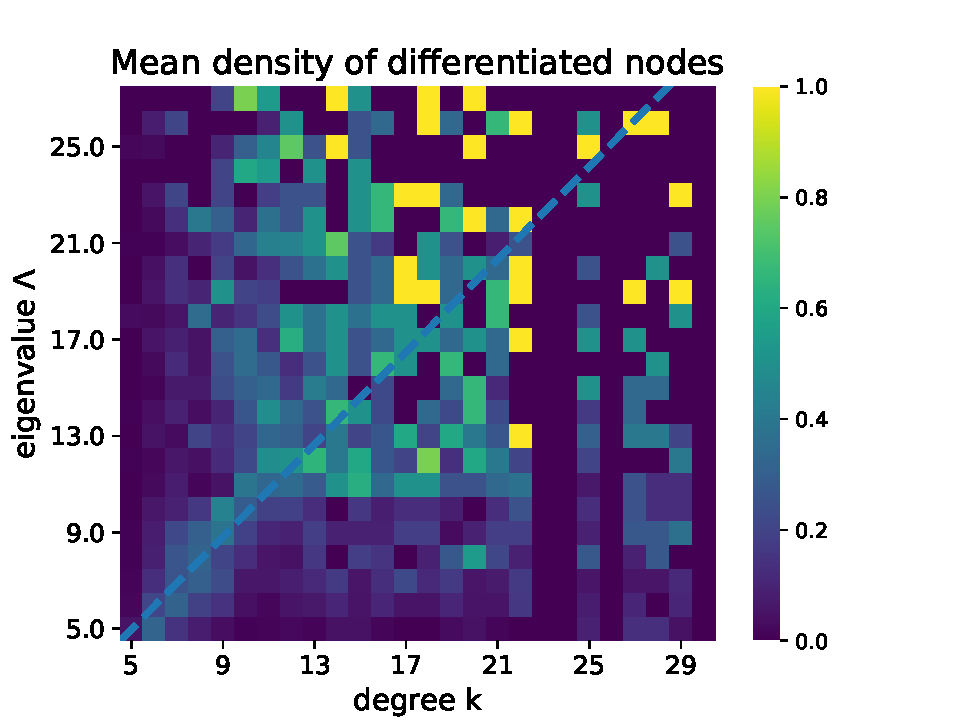
\includegraphics[width=0.48\textwidth]{latex_source/images/turing/density_200.pdf}}
\subfigure[]{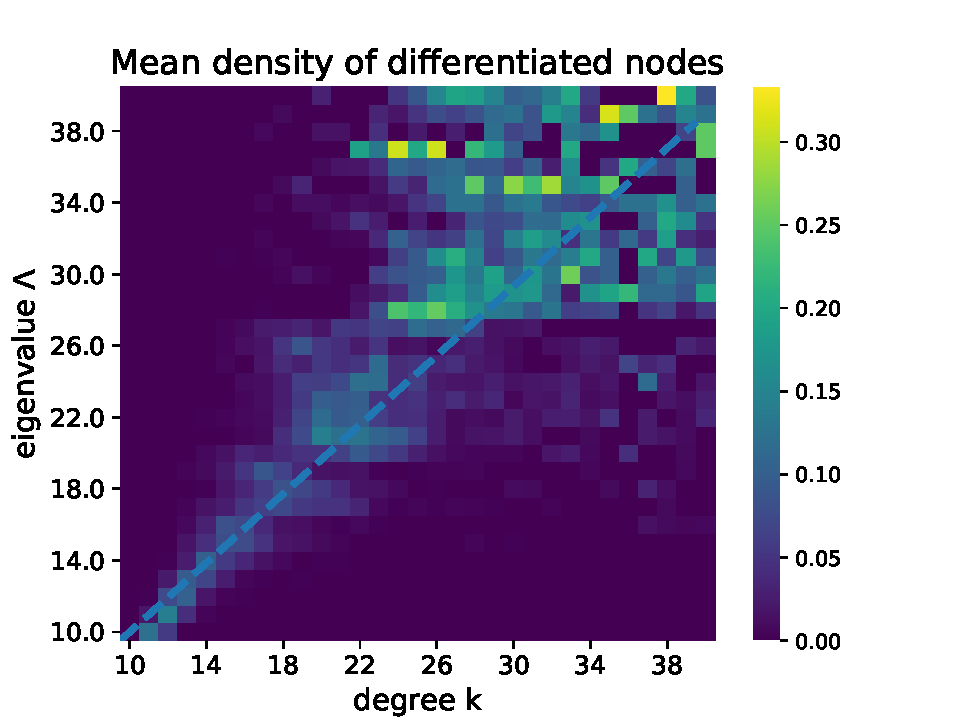
\includegraphics[width=0.48\textwidth]{latex_source/images/turing/density_1000.pdf}}
\caption{Localization of laplacian eigenvectors in a BA graph with $N=200$ nodes and $\<k\>=10$ (a) and in a BA graph with $N=1000$ nodes and $\<k\>=20$ (b). Eigenvalues have been grouped into bins of unitary width. The population of nodes inside each degree group, $N_k$, was calculated. The heatmap represents the mean density of differentiated nodes for each degree group $z = N_k^{\text{diff}}(\Lambda)/N_k$. A node $i$ of degree was considered to be differentiated with respect to eigenvalue $\Lambda_n$ if its eigenvector component satisfied, $|\Phi_i^{(n)}|> 0.1$. I found, like authors \cite{main_network} report, that approximately $\overline{k}(\Lambda) \propto \Lambda$ (dashed line) and that effect is more pronounced in the larger graph.}
\label{fig:heatmap}
\end{figure}

\nocite{bio_article}
\nocite{murray}
\nocite{altbook}
\newpage
\subsection*{Appendix}
\addcontentsline{toc}{section}{Appendix}
\textbf{Linear Stability of a 2x2 autonomous system}
\label{app:bifurcation_diagram}
Say $(\overline{x},\, \overline{y})\in \mathbb{R}^2$ is a fixed point (or equilibrium) of the autonomous system 
\begin{equation*}
    \begin{pmatrix}
        \dot{x}(t) \\
        \dot{y}(t) \\
    \end{pmatrix}
    = 
        \begin{pmatrix}
        f[x(t),\, y(t)] \\
        g[x(t),\, y(t)] \\
    \end{pmatrix}
\end{equation*}
which, namely, means that $f(\overline{x},\, \overline{y}) = g(\overline{x},\, \overline{y}) = 0$. Now we want to study how the system evolves if a small perturbation $(\delta x,\, \delta y)$ is added to the equilibrium. We can linearize the system:
\begin{equation*}
    \begin{pmatrix}
        \delta\,\dot{x}(t) \\
        \delta\,\dot{y}(t) \\
    \end{pmatrix}
    = 
        \begin{pmatrix}
        \frac{\delta\,f}{\delta x}|_{(\overline{x},\,\overline{y})} & \frac{\delta\,f}{\delta y}|_{(\overline{x},\,\overline{y})}\\
        \frac{\delta\,g}{\delta x}|_{(\overline{x},\,\overline{y})} & \frac{\delta\,g}{\delta y}|_{(\overline{x},\,\overline{y})} \\
    \end{pmatrix}
    \cdot
        \begin{pmatrix}
        \delta\,x(t) \\
        \delta\,y(t) \\
    \end{pmatrix}
    +
    o(||(\delta\,x, \delta\,y)||)
\end{equation*}
 The latter is a homogeneous linear system with general solution:
\begin{equation*}
        \begin{pmatrix}
        x(t) \\
        y(t) \\
    \end{pmatrix}
     = 
     \alpha_1 \mathbf{v}_1\, e^{\lambda_1\, t} + \alpha_2 \mathbf{v}_2\, e^{\lambda_2\, t} 
\end{equation*}
where $\lambda_1,\, \lambda_2$ are the eigenvalues of the jacobian and $\mathbf{v}_1\, \mathbf{v}_2$ are the corresponding eigenvectors, and $\alpha_1, \alpha_2$ are coefficients determined by the initial condition. The eigenvalues of a $2\cdot 2$ matrix can be both real or complex cooniugates ($\lambda_1 = \lambda, \, \lambda_2 = \overline{\lambda}$). Wether the amplitude of the perturbation dies out exponentially or explodes depends on the sign of $\mathcal{R}e\{\lambda\}$. The linear stability requirement is
$$
\mathcal{R}e\{\lambda\} <0 \quad \text{for both} \, \lambda\text{'s}
$$
The eigenvalues $\lambda_1,\, \lambda_2$ are the roots of the characteristic polynomial of the jacobian $J$:
\begin{equation*}
    p_J(\lambda) = (\lambda - \lambda_1)\cdot (\lambda - \lambda_2) = \lambda^2 - \text{tr}[J]\cdot\lambda + \text{det}[J]
\end{equation*}
\begin{minipage}{0.5\textwidth}
Then we have the following cases, depending on the discriminant $\Delta^2 = \text{tr}[J]^2 - 4\,\text{det}[J]$:
\begin{equation*}
    \begin{cases}
        \Delta^2 > 0: \quad \lambda_1,\, \lambda_2  =  \frac{\text{tr}[J] \pm \Delta }{2} \quad \text{real, distinct} \\
        \Delta^2 = 0: \quad \lambda_1,= \lambda_2 = \frac{\text{tr}[J]}{2} \in \mathbb{R} \\
        \Delta^2 <0: \quad \lambda_1,= \lambda_2  = \alpha \pm i \beta \in \mathbb{C}
    \end{cases}
\end{equation*}
One can easily see from the polynomial $p_J(\lambda)$ that in the case $\Delta^2 \geq 0$, the requirement that both roots are negative is satisfied if and only if $\text{tr}[J]<0,\, \text{det}[J] >0$. In the case $\Delta <0$, we have obligatorily $\text{det}[J] = \lambda \cdot \overline{\lambda} = |\lambda|^2 >0$, and $\text{tr}[J]= 2\cdot \mathcal{R}e(\lambda)$. Then again the requirement holds if and only if $\text{tr}[J]< 0$.
\end{minipage}
\hfill
\definecolor{mygreen}{RGB}{38, 181, 124}
\begin{minipage}{0.4\textwidth}
\centering
    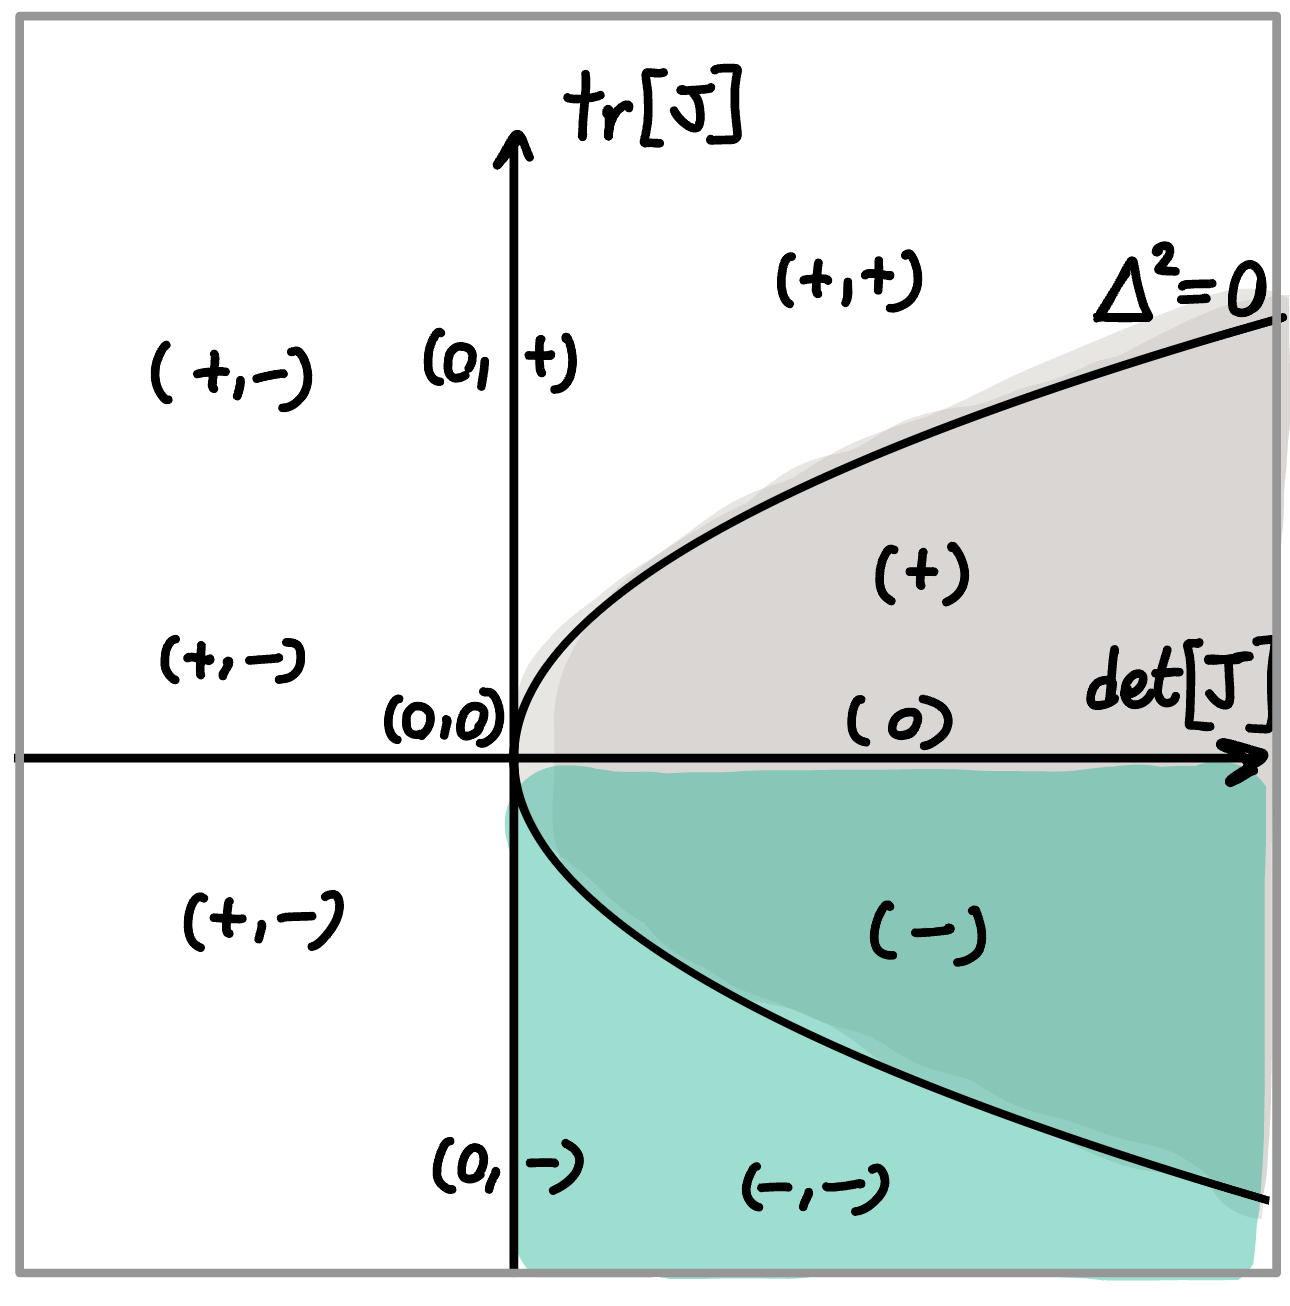
\includegraphics[width=\linewidth]{latex_source/images/turing/bifurcation.jpeg}
    \captionof{figure}{Bifurcation diagram for a $2\cdot\,2$ homogeneous system. $(\pm,\,\pm)$ are the signs of $\mathcal{R}e\{\lambda\}$ in the various regions of the (tr[J], det[J]) plane. \textcolor{mygreen}{Green} marks the stability region and \textcolor{Grey}{Grey} marks the region where eigenvalues are complex.}
    \label{fig:bifurcation}
\end{minipage}
\chapter{Task 01: Ising Model}
\section{Task Description}
The aim of this task is to simulate the Ising dynamics on complex networks. 
\section{Mathematical Model}
The ferromagnetic Ising model on a network of $N$ nodes and adiacency matrix $A$ is described in its most general form by the hamiltonian:
\begin{equation*}
    \mathcal{H}\{\mathbf{s}\} = - \sum_{i < j}\, J_{i,j}\,s_i\cdot s_j - \sum_{i}\, h_i\,s_i
\end{equation*}
where $\mathbf{s} = (s_1, \cdots s_N)$, $s_i = \pm 1$ is the spin configuration of the nodes, the couplings $J_{i,\,j}$ describe the pairwise spin interactions and $h_i$ is a site-dependent external field.
In the following, it will be always assumed $J_{i,\,j} \equiv 1\cdot A_{i,\,j}$ (only nearest neighbours interactions of homogeneous strength) and $h_i \equiv h$ (homogeneous external field), so that the hamiltonian becomes
\begin{equation}
        \mathcal{H}(\mathbf{s}) = - \sum_{i < j}\, A_{i,j}\,s_i\cdot s_j - h\cdot \sum_{i}\,s_i
\end{equation}
The network is surrounded by a heat bath at temperature $T = \frac{1}{\beta} $ ($k_B \equiv 1$). The partition function $Z$ and the free energy $F$ are given by:
\begin{equation*}
    Z\left(T, \{A_{i,\,j}\}, h, N\right) = \sum_{\mathbf{s}}\, e^{-\beta\, \mathcal{H}(\mathbf{s})} \quad F = -\frac{1}{\beta}\, \text{ln}[Z]
\end{equation*}
The most relevant thermodynamic quantities are the internal energy $E$, the magnetization $M$, the specific heat $C$ and the magnetic susceptibility $\chi$:

\begin{align*}
E &= \mathbbm{E}[\mathcal{H}(\mathbf{s})], &
C &= \left( \frac{\partial E}{\partial T} \right)_{h} \equiv \frac{\mathbbm{E}[E^2] - \mathbbm{E}[E]^2}{T^2} \\
M &= \mathbbm{E}\left[\sum_{i} s_i \right] \equiv \left( \frac{\partial F}{\partial h} \right)_{\beta}, &
\chi &= \left( \frac{\partial M}{\partial h} \right)_{T} = -\left( \frac{\partial^2 F}{\partial^2 h} \right)_{T} \equiv \frac{\mathbbm{E}[M^2] - \mathbbm{E}[M]^2}{T^2}
\end{align*}


\noindent By means of a mean field approximation, it is possible to show that the existence of a disordered phase depends on the moments $\left\langle k^n\right\rangle$ of the degree distribution. Specifically, a homogeneous mean field approximation yields the critical temperature
\begin{equation} \label{eq:hom_mean_field}
    T_C^{\text{hom. MF}} =\,\left\langle k \right \rangle
\end{equation}
 ([Appendix \ref{app:mean_field}] contains the explicit calculations for this formula), while the more accurate heterogeneous (or degree-based) mean field approximation yields:
\begin{equation} \label{eq:het_mean_field}
    T_C^{\text{het. MF}} =\,\frac{\left\langle k^2 \right \rangle}{\left\langle k \right \rangle}
\end{equation}
In particular, the latter formula is derived under the assumption that the network is uncorrelated, that is, the nearest neighbour degree distribution is the same as in the configuration model $P_{n.n.} (k)=\frac{k\cdot P(k)}{<k>}$.
A refined estimation of the critical temperature is found with the replica approach \cite{analytical_ising}. \\ 
\begin{equation}
    T_C^{replica} = \left[ -\frac{1}{2}\,\text{ln}\left[2- \frac{\left\langle k \right\rangle}{\left\langle k^2 \right\rangle}\right]\right]^{-1}
\label{eq:replica}    
\end{equation}
The order parameter of the transition is the average magnetization per site, $s$:
$$
s := \frac{M}{N} = \mathbbm{E}\left[\frac{\sum_{i}\,s_i}{N}\right]
$$
which is zero in the disordered phase ($T>T_C$), non-zero in the ferromagnetic  phase $(T<T_C)$ and monotonically decreasing with temperature. Also, the energy $E(T)$ is expected to have an inflection point at $T=T_C$, and the response function $C$ and $\chi$ are both supposed to peak at $T=T_C$.

\section{Numerical Simulations}
For simulations, I chose to focus on scale free networks $P(k) \sim k^{-\gamma}$, in particular the Barabasi - Albert (BA) network of parameters $N,\, m$ where N is the number of nodes and $m$ is the number of links attacched for each new node. This choice was motivated by the fact that article \cite{numeric_ising} could be used for comparison. The degree distribution for such a network is asymptotically given by $P(k) \sim k^{-3}$. Since one can only deal with finite size networks, finite size effects must be taken into account in the formulas $[\ref{eq:hom_mean_field}$, $\ref{eq:het_mean_field}, \ref{eq:replica}$.
The finite size of the network implies the existence of a cutoff degree $k_{max}(N)$, so the right estimation of the moment $\left\langle k^n \right \rangle$ is given by
\begin{equation*}
    <k^n> = \sum_{k=m}^{k_{max}(N)}\, k^n\,P(k)
\end{equation*}
where the cutoff $k_{max}(N)$ is defined such that the probability of having a node of degree $k>k$ in a network of size $N$ is less than one. With an elementary calculation one can verify that $k_{max}(N)= m\cdot N^{\frac{1}{\gamma -1}}$, which reduces to $k_{max} = m\cdot \sqrt{N}$ for a BA network.
The average degree is left unchanged by the finite size correction:  $<k> = 2m$, whereas the second moment changes to $<k^2> \simeq m^2\,\text{ln}(N)$ \cite{analytical_ising}. Hence, the critical temperatures given by the mean field formulas are:
\begin{equation}
    T_C^{\text{hom. MF}} = 2m, \quad \quad T_C^{\text{het. MF}} \simeq \frac{m}{2}\,\text{ln}(N)
\end{equation}
The heterogeneous mean field approximation predicts a logaritmic increase of the temperature with the network size, which means that in the thermodynamic limit ($N\rightarrow +\infty$) the network is expected to be ferromagnetic at all temperatures. The homogeneous mean field is too drastic and fails to predict this behaviour. Additionally, these formulas state that the critical temperature is expected to increase with the average degree, which indicates that adding more connections between the nodes helps in mantaining long-range order.
\bigskip \newline \noindent
The algorithm I implemented to simulate the Ising dynamic is the Metropolis-Hasting. As a preliminary check, I used my code to simulate the Ising model on a regular $2d$ lattice of $N =400$ nodes [Appendix, figures: \ref{fig:2d_relaxation} and \ref{fig:2d_scaling}]. Then I moved on to BA networks.
Computational cost for the simulations on BA was much higher than for a 2d regular lattice of the same size. Handling the adiacency matrix of the network in sparse format brought a significant performance improvement, but still the computations were long (for comparison, obtaining the scaling of lattice quantities with temperature [Appendix, figure: \ref{fig:2d_scaling}] took $12$ minutes, whereas obtaining the same data for BA [Figure: \ref{fig:BA_scaling_m_10}] took on average $\sim 1h$). \medskip \newline \noindent
 For the estimation of the critical temperature, I first considered extracting one estimation out of each of the four thermodyninamic quantities ($E, \left\langle s \right\rangle , C, \chi$) and then average them. However, I found that the peak temperature of the specific heat $C$ was sistematically lower than the peak temperature for the magnetic suscepitibility $\chi$ [see Figure: \ref{fig:BA_scaling}]. The latter was closer to the theoretical expected temperature value. This behaviour was not found in the preliminary simulation on a $2d$ regular lattice, thus I can exclude that it is an artifact of my code. In fact, I became avare the same behaviour has been observed by my colleague D.Wellingut \cite{dw}.
\begin{figure}[H]
    \centering
    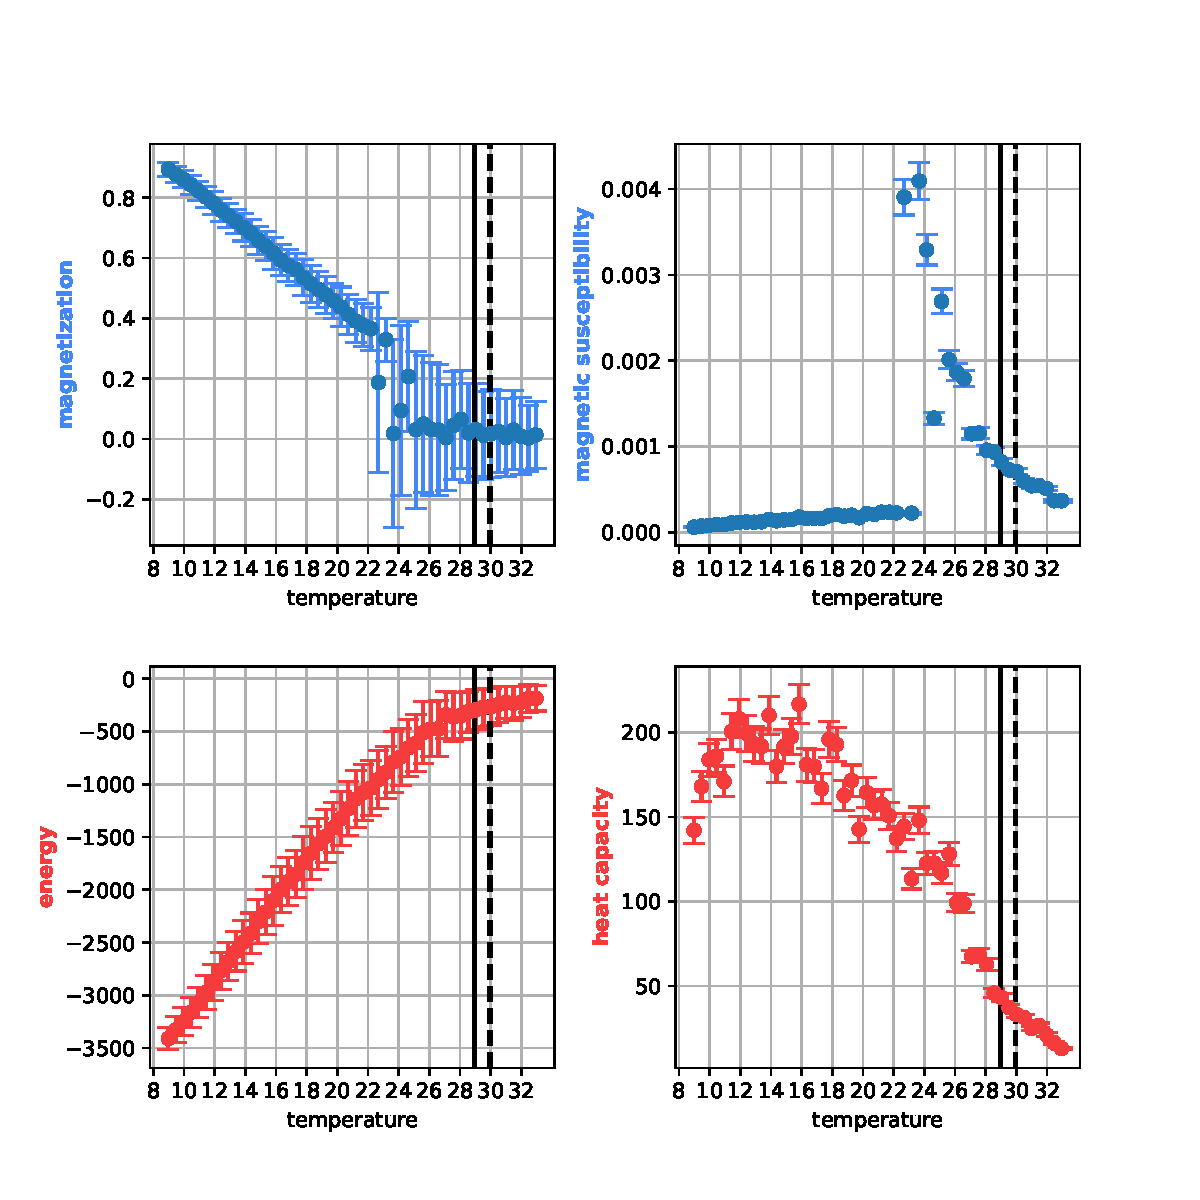
\includegraphics[width=0.85\linewidth]{latex_source/images/ising/BA_scaling_num_nodes_400_t_points_50_steps_700_m_10_ti_8.99_tf_32.95.pdf}
    \caption{Scaling of thermodinamic quantities with temperature. BA network with $N=400$ and $m=10$. Metropolis algorithm was run with $1500$ equilibration steps and $700$ sweep steps. The dashed line is the heterogeneous mean field temperature \ref{eq:het_mean_field}, while the solid line is the replica temperature \ref{eq:replica}. The peaks of the two response fuctions do not coincide.}
    \label{fig:BA_scaling_m_10}
\end{figure}
\noindent For this reason, I only averaged the temperatures obtained from the magnetization and the magnetic susceptibility, disregarding the other two. The final results of my simulations are shown in [Figure: \ref{fig:final_ising}]. The critical temperature estimated from the simulations is systematically lower than the theoretical predictions, but at least the dependence on $m$ is similiar.
\begin{figure}[H]
    \centering
    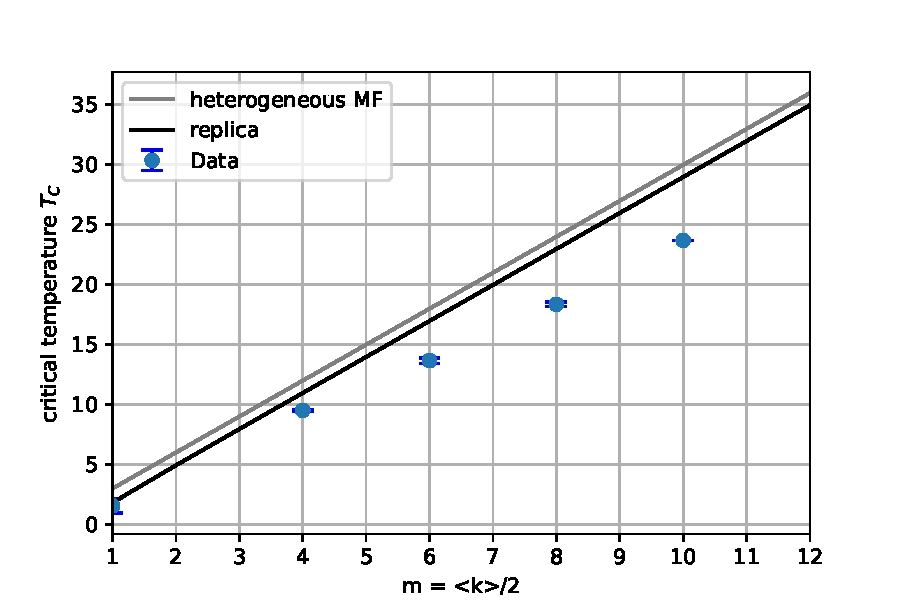
\includegraphics[width=0.8\linewidth]{latex_source/images/ising/BA_temperatures.pdf}
    \caption{Scaling of the critical temperature with the minimum degree, for BA networks of $400$ nodes. The data refer to the critical temperature estrapolated from the magnetization and the magnetic susceptibility peak.}
    \label{fig:final_ising}
\end{figure}

\newpage
\section*{Appendix}
\addcontentsline{toc}{section}{Appendix}
\subsection*{Mean-field $T_C$ calculation} \label{app:mean_field}
{\small
The mean field approximation consists in negletting the pairwise spin correlations $
    \text{corr}(s_i,\,s_j) = (s_i - \left\langle s_i \right \rangle)\cdot (s_j - \left\langle s_j \right \rangle)\simeq 0 $.
Moreover, the homogeneous mean field supposes that the average magnetization on each node is the same for all nodes $\left\langle s_i\right\rangle \equiv \left \langle s \right \rangle$, while the heterogeneous mean field makes the weaker assumption that the average magnetization on a node depends at most on the node's degree: $\left \langle s_i\right \rangle \equiv \left\langle s_{k_i}\right\rangle$. 
Let's consider the homogeneous mean field for simplicity. \medskip \newline \noindent
We start from the hamiltonian $H\{\mathbf{s}\} = -\frac{1}{2}\, \sum_{i,\,j}\,A_{i,\,j}\,s_i\cdot s_j - h\cdot\sum_{i}\,s_i$ and write the identity 
\begin{align*}
    s_i\cdot s_j &= [s_i - \left\langle s \right \rangle + \left\langle s \right \rangle]\cdot [s_j - \left\langle s \right \rangle + \left\langle s \right \rangle] \\
    &= (s_i - \left\langle s \right \rangle)\cdot (s_j-\left\langle s \right \rangle) + (s_i + s_j) \left\langle s \right \rangle - \left\langle s \right \rangle^2 \simeq (s_i + s_j) \left\langle s \right \rangle - \left\langle s \right \rangle^2
\end{align*} where the latter is obtained disregarding the correlation term. With this substitution, the hamiltonian becomes 
\begin{equation*}
    H \simeq\frac{1}{2}\,\left\langle s \right \rangle^2\,N\,\left\langle k \right \rangle - \sum_i\,s_i\cdot (\left\langle k \right \rangle\left\langle s \right \rangle + h)=: H^{MF}(\mathbf{s})
\end{equation*}
This expression can be now used to compute the partition function $Z$ and, consequently, the free energy per site $f= F/N$:
\begin{align*}
    Z^{MF} &= \sum_{\mathbf{s}}\, e^{-\beta H^{MF}(\mathbf{s})} = e^{-\beta \frac{N \left\langle k \right \rangle\left\langle s \right \rangle^2}{2}}\, \sum_{\mathbf{s}}\, e^{\beta\left[(<k><s> + h)\sum_l\,s_l\right]} \\
    &= e^{-\beta \frac{N <k><s>^2}{2}}\, \prod_{i=1}^{N}\, \left[ \sum_{s = \pm 1}\, e^{\beta(<k>+h)\,s_i} \right] \\
    &= e^{-\beta \frac{N \left\langle k \right \rangle\left\langle s \right \rangle^2}{2}}\,\left[2\,\text{cosh}\left[\beta(\left\langle s \right \rangle\left\langle k \right \rangle+h)\right]\right]^N \\
   f^{MF}&= \frac{F^{MF}}{N} = - \frac{1}{N\beta}\text{ln}Z^{MF} = \frac{1}{2}\left\langle k \right \rangle\left\langle s \right \rangle^2 -\frac{1}{\beta}\text{ln}\left[2\,\text{cosh}[\beta(\left\langle s \right \rangle\,\left\langle k \right \rangle+h)]\right]
\end{align*}
The average magnetization per site is then given by
\begin{equation*}
    <s> = -\left(\frac{\partial f^{MF}}{\partial h}\right)_\beta = (\cdots) = \text{tanh}[\beta(<s><k>+h)]
\end{equation*}
When the external field is off, $\left\langle s\right\rangle$ solves the self consistent equation $\left\langle s\right\rangle = \text{tanh}[\beta\,\left\langle s\right\rangle\,\left\langle k\right\rangle]$, which is the interesection of $y = \left\langle s\right\rangle$ and $y = \text{tanh}[\beta\,\left\langle s\right\rangle\,\left\langle k\right\rangle]$.
For $\beta < \beta_C = \frac{1}{\left\langle k\right\rangle}$, there are no intersection points other than $\left\langle s \right \rangle = 0$  ($\Rightarrow$ the system is paramagnetic) for $\beta > \beta_C$ there are two simmetric non-zero intersections ($\Rightarrow$ the system is ferromagnetic). The critical temperature is thus given by $T_C = \frac{1}{\beta_C} = \left\langle k \right\rangle$, which is exactly [Eq. \ref{eq:hom_mean_field}].
\begin{figure}[H]
    \centering
    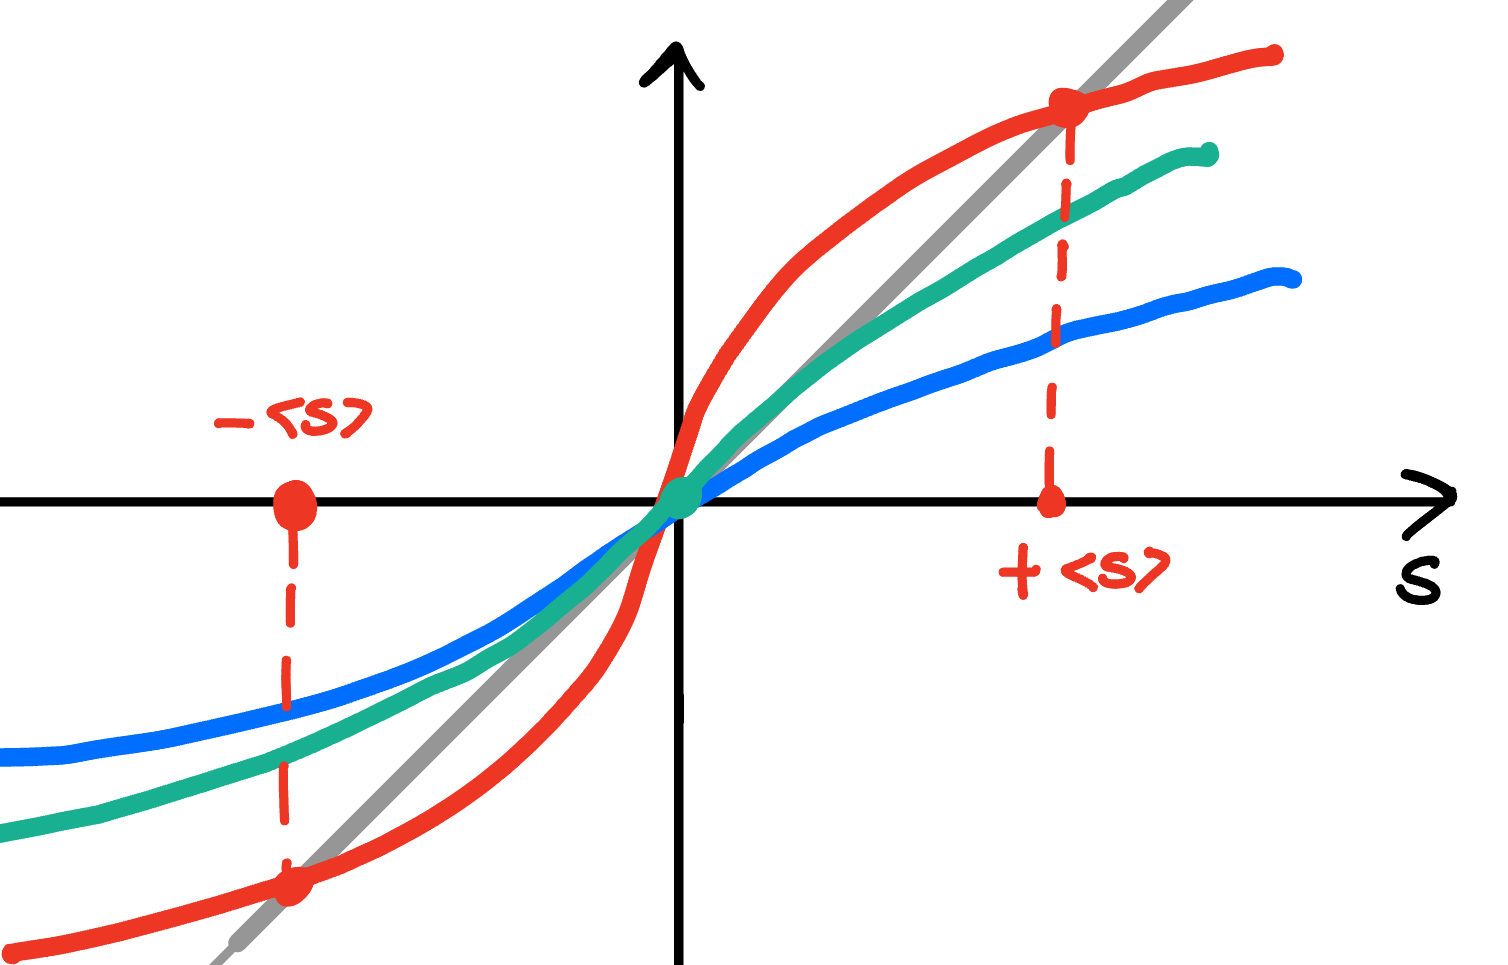
\includegraphics[width = 0.4\textwidth]{latex_source/images/ising/IMG_56FE6CFC861B-1.jpeg}
    \caption{\small Grey line is $y=s$, coloured lines are $y = \text{tanh}(\beta \left\langle k\right\rangle s)$, respectively for $\beta \left\langle k\right\rangle  > 1$ (red, ferromagnetic state), $\beta \left\langle k\right\rangle > 1$ (green, critical point) and $\beta \left\langle k\right\rangle < 1$ (blue, paramagnetic state).}
\end{figure}
\subsection*{Preliminary Montecarlo simulation on a 2D lattice}
{\small
An infinite regular $2-$ dimentional spin lattice exibits a second order phase transition at the critical temperature 
\begin{equation}
T_C = \frac{2\,}{\,\log{1 + \sqrt{2}}} \simeq 2.26
  \end{equation}  
    \label{eq:onsager}
For my simulation, I considered a lattice of $N = 20 \cdot 20 = 400$ nodes. I first simulated the dynamics at fixed temperature, to get an estimate of the number of steps required for the system to equilibrate. I found that $\simeq 500$ steps where sufficent for a lattice of this size [Fig \ref{fig:2d_relaxation}]. Then I simulated Ising over a broad range of temperatures around the expected critical temperature and computed the energy, magnetization, heat capacity and magnetic susceptibility [Fig: \ref{fig:2d_scaling}].
}
\begin{figure}[H]
    \centering
    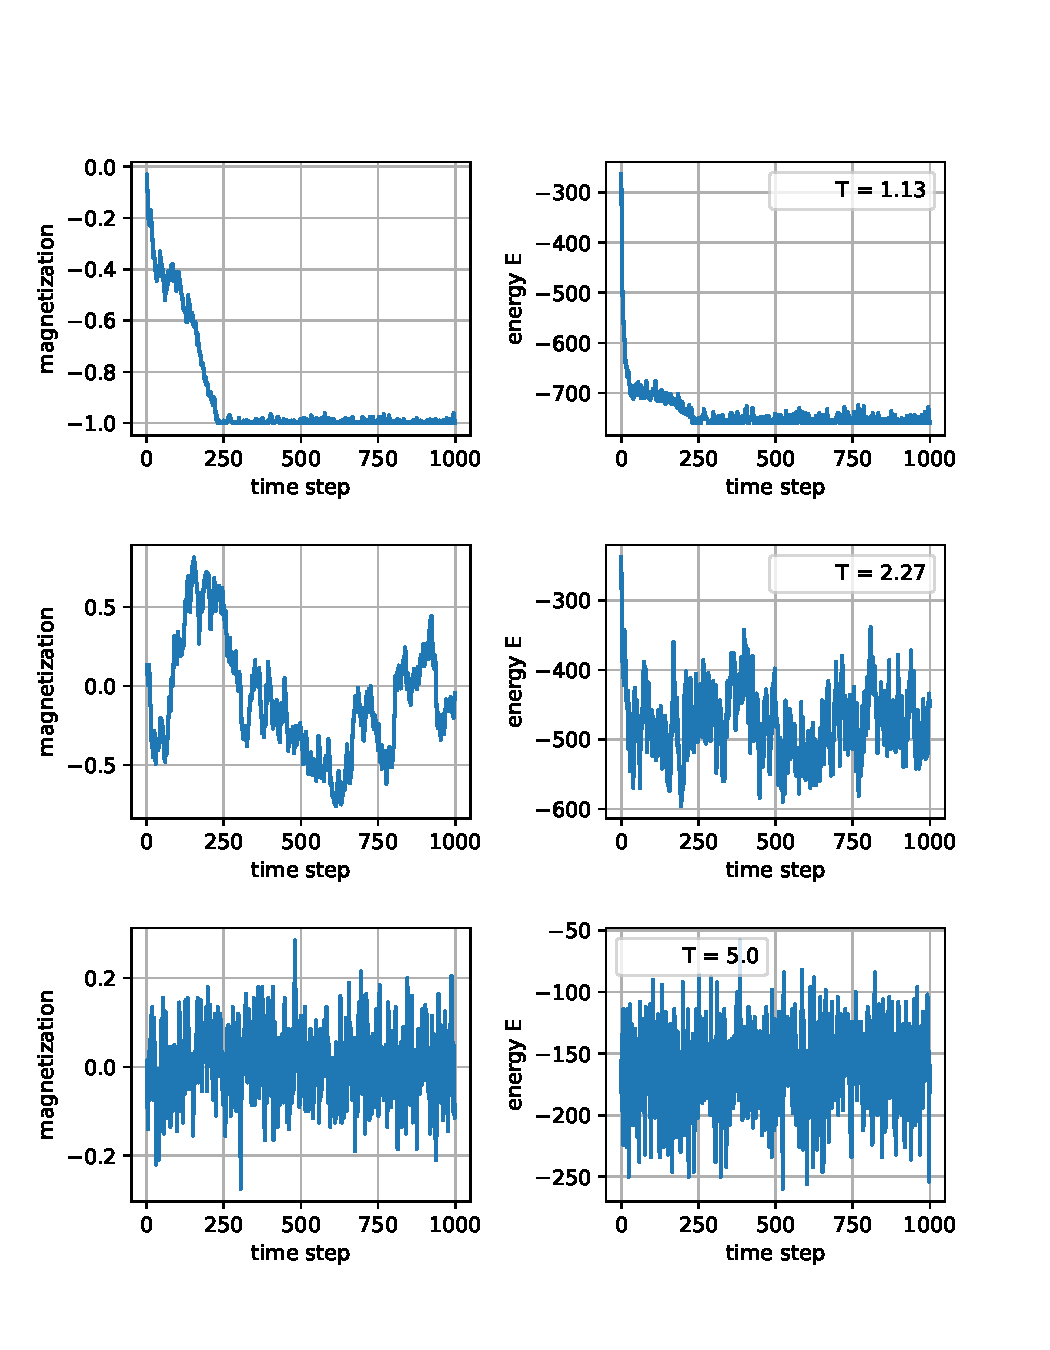
\includegraphics[width=0.8\linewidth]{latex_source/images/ising/2d_relaxation.pdf}
    \caption{{\small Time evolution of the magnetization and energy, respectively below, at and above the critical temperature \ref{eq:onsager}. Approximately $\sim\,250$ Metropolis steps are enough for the sistem to equilibrate.}}
    \label{fig:2d_relaxation}
\end{figure}

\begin{figure}[H]
    \centering
    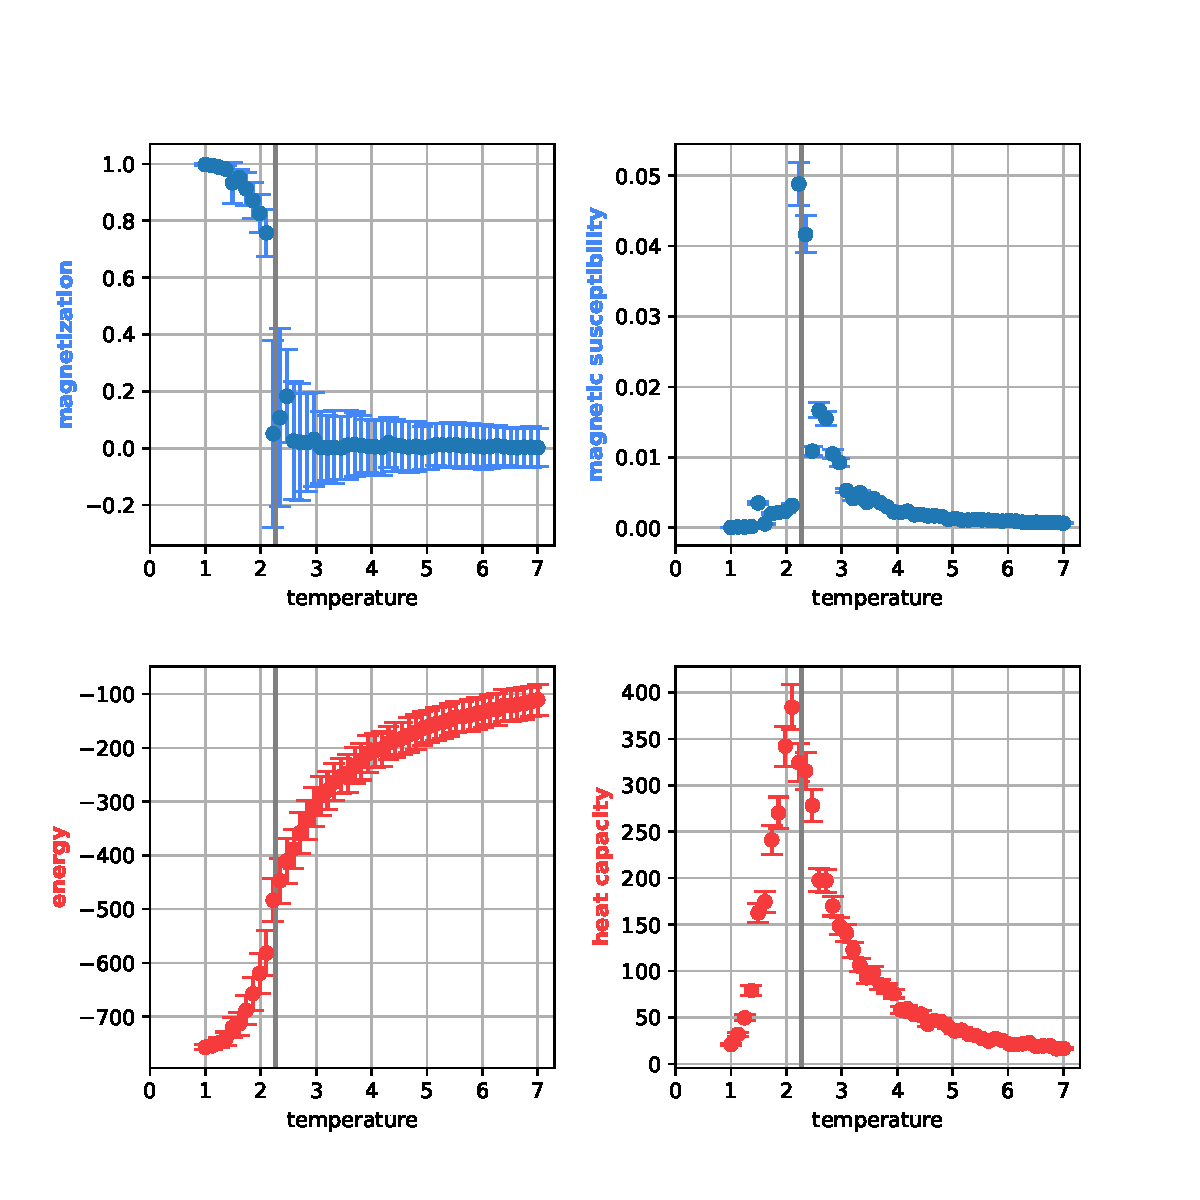
\includegraphics[width=\linewidth]{latex_source/images/ising/2d_scaling.pdf}
    \caption{Dependence of thermodynamic quantities on temperature. The vertical grey line marks the theoretical critical temperature as given by Onsager's formula [Eq: \ref{eq:onsager}]. One can see that the peaks of $C$ and $\chi$ are very close to the theoretical temperature. For $500$ equilibration steps and $500$ sweep steps at each temperature, the code took $12$ minutes to execute.}
    \label{fig:2d_scaling}
\end{figure}
}
\chapter{Task 28: Voter Model}

\section{Task Description}
The voter model is perhaps the simplest and most studied model of cooperative behaviour. While its behaviour on regular lattices of arbitrary dimention $d$ is known in detail, it is much more difficult to get a comprehnsive general picture of its behaviour on a complex network, where there is interplay between many factors, such as the degree distribution, the effective dimentionality, the degree of disorder, the presence of correlations \cite{suchecki_numerical}. 
The aim of this task is to describe the voter model and attempt to reproduce its behaviour on some class of networks. Specifically, I chose to focus on scale free networks, for which some analitical results have been found \cite{sood}. 

\section{Mathematical Model}
In the voter model, each node of the network is in one of two possible states, say, spin up or spin down: $\sigma_i \in \{\pm 1\}$. The evolution starts with some random configuration of up and down spins. The update rule is defined as follows: 
\medskip
\newline
\begin{minipage}{0.8\textwidth}
\begin{itemize}
    \item[i)] choose one node at random,
    \item[ii)] choose one of its neighbors at random,
    \item[iii)] ascribe to this node the current state of its neighbour.
\end{itemize}
\end{minipage}
\hfill
\begin{minipage}{0.2\textwidth}
\vfill
    \textit{Node-update rule}
\vfill
\end{minipage}
\medskip
\newline
Actually, there is an alternative rule which may look equivalent:
\medskip
\newline
\begin{minipage}{0.8\textwidth}
\begin{itemize}
    \item[i)] choose one link at random,
    \item[ii)] choose one of its ends at random,
    \item[iii)] ascribe to this node the current state of the other end.
\end{itemize}
\end{minipage}
\hfill
\begin{minipage}{0.2\textwidth}
\vfill
    \textit{Link-update rule}
\vfill
\end{minipage}
\medskip
\newline
Indeed the two rules are equivalent for regular lattices, but not in the case of complex networks \cite{suchecki_analitical}. For each time step, this update rule is applied $N$ times if $N$ is the network size, so that \textit{on average} each node is updated once. The voter model defines a markovian stochastic process. There are two absorbing states: all spins up and all spins down (when it reaches one of these states, it cannot change anymore, that is why they are called absorbing). If we identify network nodes as people and spin up and down with two possible opinion, the absorbing state represent consensum. \\
There is always a chance that a finite size network reaches consensus. In fact, \textbf{the mean time to reach consensus in a finite network is always finite} (the mean is here intended over the set of all evolution histories and initial conditions), whether it is a regular lattice or a complex network. However, conceptually there are different scenarios when infinite size networks are considered instead.\\
The mean time $\left \langle \tau \right \rangle$ to reach consensus in a finite, regular lattice of $N$ nodes and dimention $d$ is known to scale as:
\begin{equation*}
    \left \langle \tau \right \rangle(N) \sim
    \begin{cases}
        N^2 \quad &\text{if}\quad d=1 \\
        N\cdot \ln{N} &\text{if}\quad d=2 \\
        N &\text{if}\quad d>2 \\
    \end{cases}
\end{equation*}
For networks, one could guess to find $\left \langle \tau \right \rangle(N) \sim N$ as for high dimentional lattices. However this is not true in general. For instance, \cite{sood} found analitically that, for uncorrelated, scale-free networks with degree distribution $P(k)\sim k^{-\gamma}$ and \textit{node-update} rule:
\begin{equation*}
    \left \langle \tau \right \rangle(N) \sim
        \begin{cases}
         N^{\alpha}, \, \alpha<1 \quad &\text{if}\quad \gamma < 3 \\
        \frac{N}{\ln{N}} &\text{if}\quad \gamma = 3 \\
         N &\text{if}\quad \gamma > 3 \\
    \end{cases}
\end{equation*}
Generically, $\tau(N)$ grows sublinearly with N; that is, high-degree nodes greatly accelerate the approach to consensus. \cite{suchecki_numerical} numerically found for Barabasi-Albert networks a scaling $\tau \sim N^{0.88}$, which is compatible with $\tau \sim \frac{N}{\ln{N}}$, and a scaling $\tau \sim N$ (like for the high dimentional lattices) when the \textit{edge-update} rule is used instead. \\
A standard order parameter used to measure the ordering process of the voter dynamic is the \textit{average interface density $\rho$}, defined as the density of edges connecting nodes with different states:
\begin{equation}
    \rho(\mathbf{\sigma}) := \frac{\sum_{i,\,j}\left[A_{i,\,j}\,\cdot \mathbbm{1}(\sigma_i,\,\sigma_j)\right]}{\sum_{i,\,j}\, A_{i,\,j}}, \quad \text{where} \, \mathbbm{1}(\sigma_i,\,\sigma_j):= \frac{1 - \sigma_i\,\sigma_j}{2} = 
    \begin{cases}
        1 & \text{if}\quad \sigma_i\neq \sigma_j \\
        0 & \text{if}\quad \sigma_i= \sigma_j \\
    \end{cases}
\label{eq:rho}
\end{equation}
\section{Numerical Simulations}
\begin{figure}[H]
    \centering
    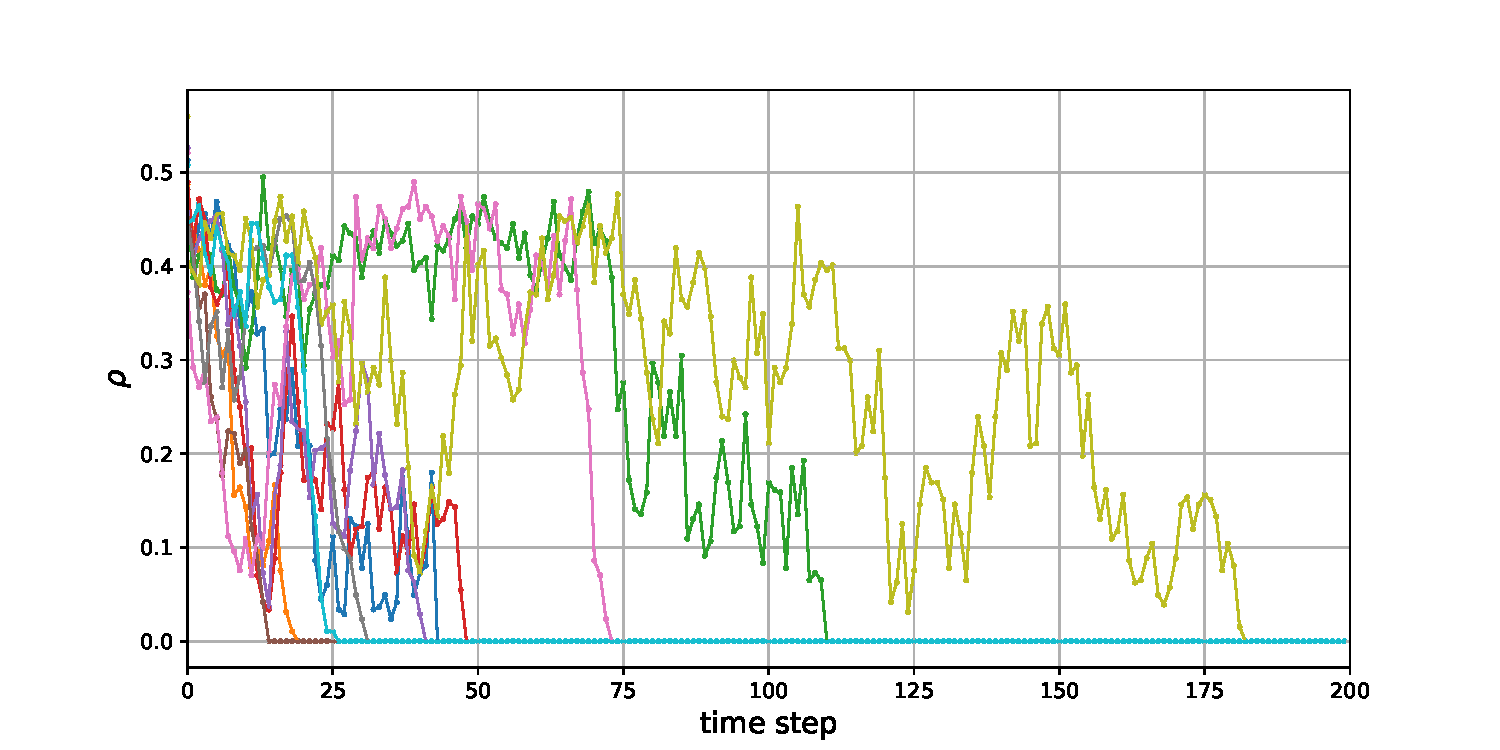
\includegraphics[width=\linewidth]{latex_source/images/voter/example_evolution.pdf}
    \caption{Evolution of the voter model on Barabasi-Albert networks with $N=100$ and $\left\langle k\right\rangle = 8$. Each line is a trajectory on a different network instance of the BA model. Initial state is drawn uniformly at random for each trajectory.}
    \label{fig:enter-label}
\end{figure}

\begin{figure}[H]
    \centering
    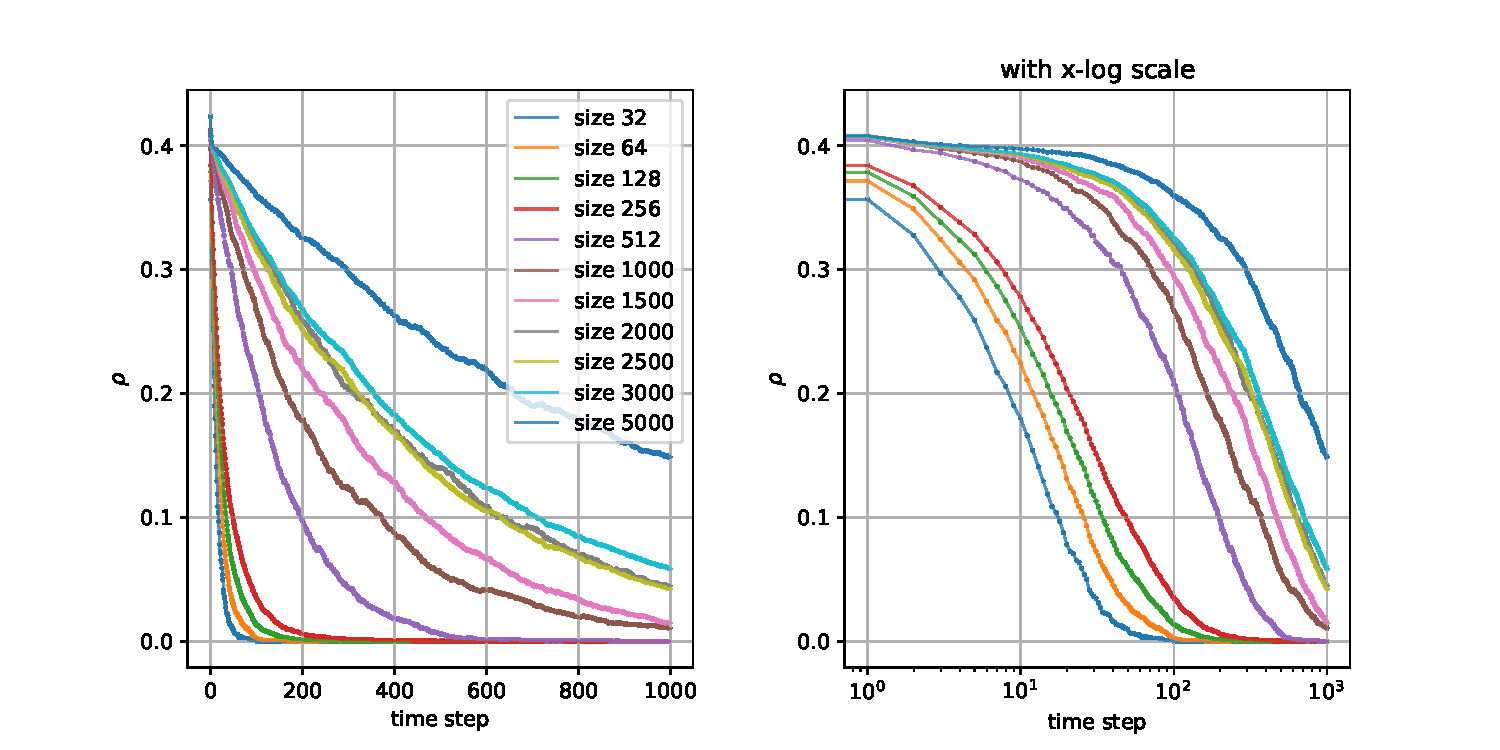
\includegraphics[width=\linewidth]{latex_source/images/voter/BA_node_update_rule_results_logscale.pdf}
    \caption{Evolution of the average interface density [Eq. $\ref{eq:rho}$] in Barabasi Albert networks of mean degree $\left\langle k\right\rangle= 6$ different sizes. Data is averaged over $500$ realizations. }
    \label{fig:BA_evolution}
\end{figure}

\begin{figure}[H]
    \centering
    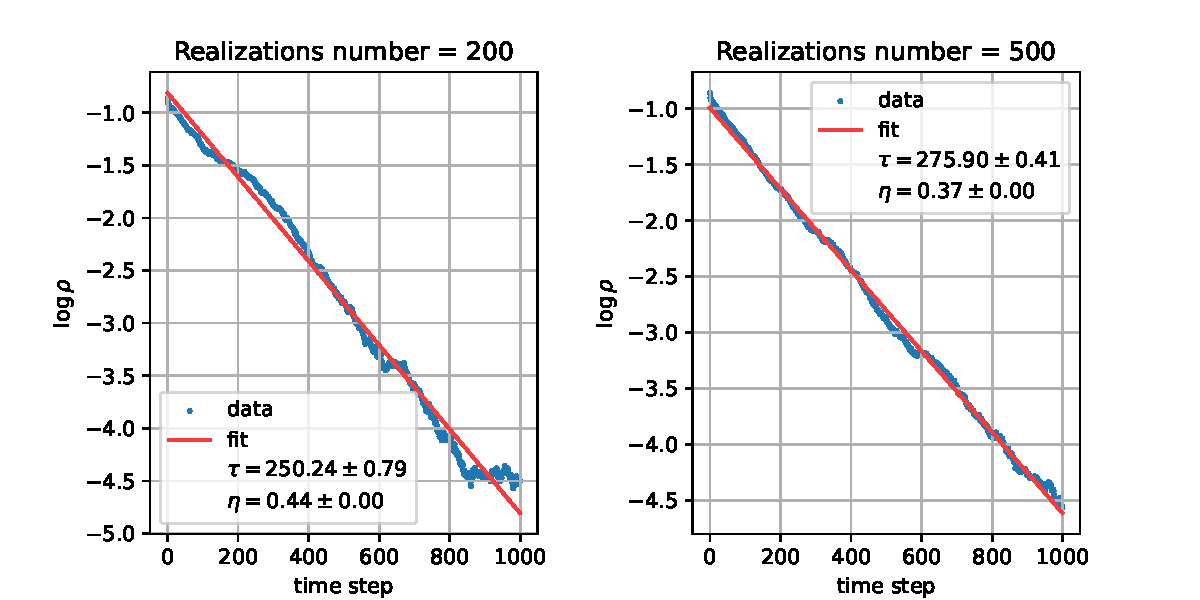
\includegraphics[width=\linewidth]{latex_source/images/voter/comparison.pdf}
    \caption{Comparison between exponential fit parameters estimated from $200$ (left) and $500$ (right) different realization on BA networks with same size $N=1000$. }
    \label{fig:enter-label}
\end{figure}

\begin{figure}[H]
    \centering
    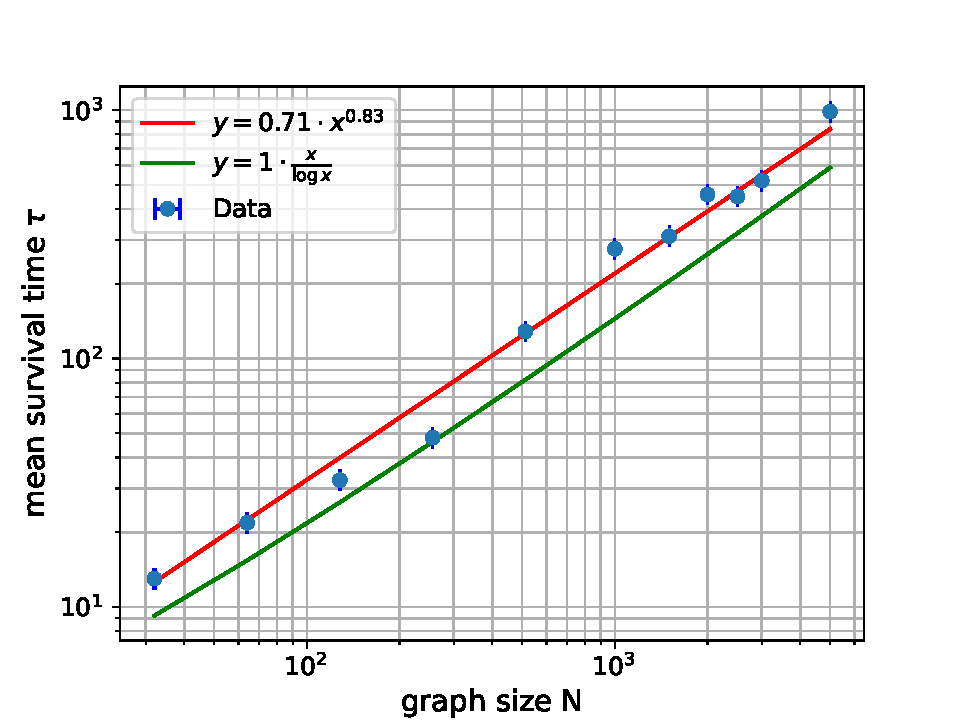
\includegraphics[width=0.7\linewidth]{latex_source/images/voter/BA_time_scaling.pdf}
    \caption{Average survival times for Barabasi Albert networks of different sizes, as results from the exponential fit of the curves in [Fig: $\ref{fig:BA_evolution}$]. Data is fitted with a power law $y = \alpha \cdot x^\gamma$ with free parameters $\alpha,\, \gamma$ with the method of least squares For comparison, also the theoretical expectation $\tau \sim \frac{N}{\log{N}}$ is plotted (green line). One can see that the slope of the two curves are very similiar.}
    \label{fig:BA_scaling}
\end{figure}
\chapter{Task 46: EU transportation network II}
\section{Task Description}
The aim of this task is to reconstruct the railway networks of European countries from the raw geographical data provided in the open database
\parencite[][ \textit{EuroGlobalMap}, $2019$ release]{euroglobalmap}. The requested output for each network is two files: one containing the edge list and one containing the node metadata \textit{[nodeLabel, latitude, longitude, country\_name, country\_ISO3]}.
\section{Data extraction}
The choice of what exactly the nodes of the network should represent is not specified (a possibility is to identify nodes with cities, but one could also opt for administrative district or even larger regions).
I decided to build networks where \textbf{nodes} correspond to \textbf{cities} where a railway station is present, and two nodes are connected through an \textbf{edge}  if they are \textbf{consecutive stops} of some rail. The accomplishment of this task was not straightforward. The best way I found involves first creating a preliminary network, where nodes do not have any specific physical significance, and, subsequently, extracting the desired network as a subset of it. \newline \noindent
I consulted \textit{EGM19\_DataSpecification.pdf, 
 Annex C - Definition of Features and Attributes} to understand what files I needed to look for in the database, Python library GeoPandas to open the shapefiles and NetworkX to create and manipulate graph objects. Station's data encoded in \textit{Point} objects containing the station's latitude and longitude, while railway data is encoded in \textit{LineString} objects, which are lists of points that connected together form a segmented line.
Besides, geometrical data comes with a number of attributes. These include :'ICC', the 2- character country IS03 code (es. IT, for Italy),  'NAMA1', the station name, and 'EXS', the existence category of the rail (e.g. abandoned, operational, under construction...).
\medskip \newline \noindent
As said already, in my method the desired networks are extracted as a subset of a preliminary network. 
The latter is built upon the data contained in file \textit{RailrdL.shp} with the following steps:
\newline \noindent
\begin{minipage}{0.5\textwidth}
\begin{enumerate}
    \item open the shapefile \textit{RailrdC.shp/.shx/.dbf} with Geopandas and extract relevant attributes
     \item initialize an empty graph with NetworkX
     \item iterate through the dataframe rows. For each LineString object, assign each of its point-like components to a node of the graph. Draw an edge between each pair of successive components.
\end{enumerate}
Figure [Fig: \ref{fig:raw}] shows what the resulting network looks like. At this stage, the nodes have no particular physical meaning: they are just the starting and ending points of the straight segments that make up the rail line.
\end{minipage}
\hfill
\begin{minipage}{0.48\textwidth}
    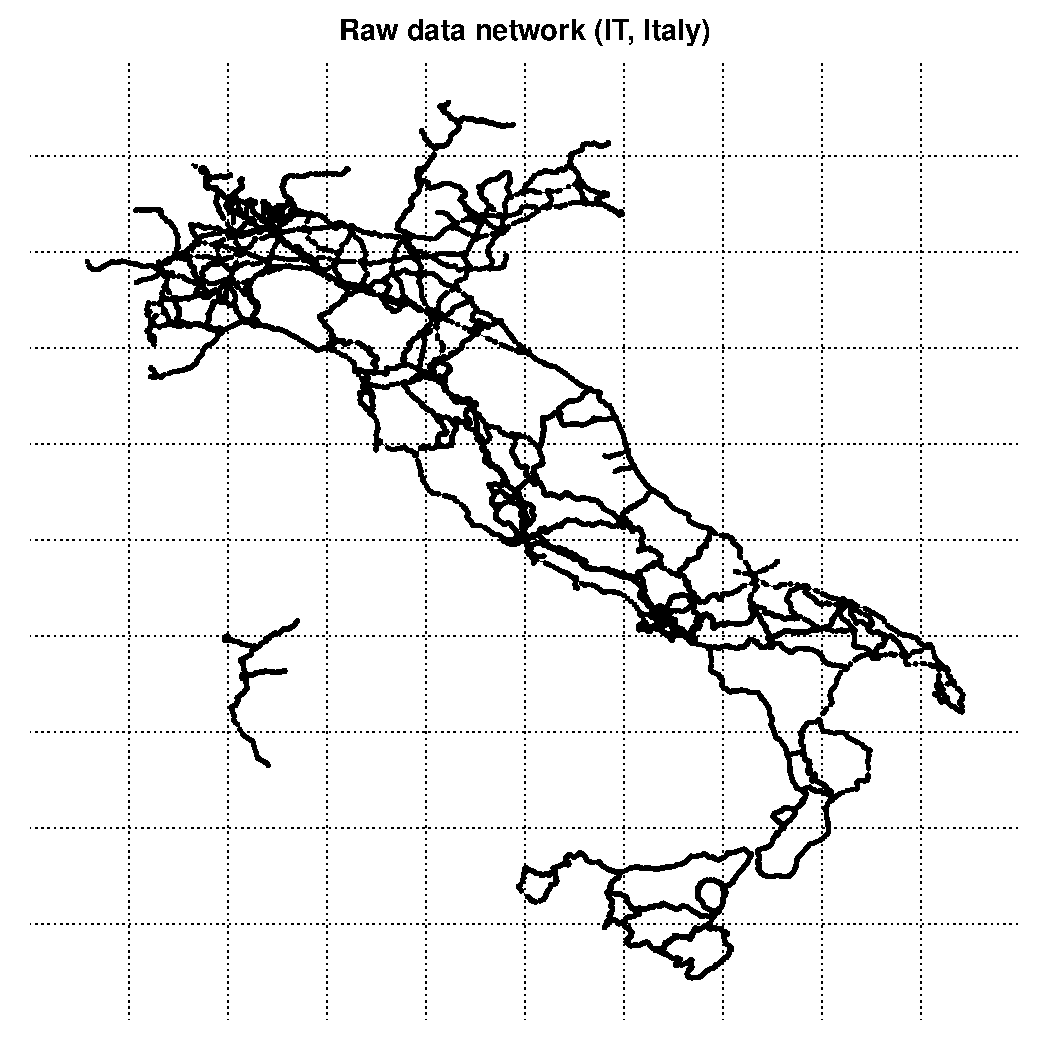
\includegraphics[width = \textwidth]{latex_source/images/railways/raw_networks/raw_IT_network.pdf}
    \captionof{figure}{}
    \label{fig:raw}
\end{minipage}
\bigskip \newline 
The following step consists in selecting only the nodes which corresponds to actual city stations, and rewire the links. To achieve this:
\begin{enumerate}
    \item city stations data is loaded from file \textit{RailrdC.shp/.shx/.dbf},
    \item \textit{Node labeling}: two new attributes are assigned to nodes of the preliminary network: "label" and "is\_near\_city". These fields are both "empty" by default.
    A loop checks if the preliminary network nodes' coordinates match any of the stations coordinates within a given threshold distance $d$. Nodes in the preliminary network are very dense, and in general more than one node will satisfy the threshold condition. The best match is assigned attribute "label = station\_name", while the others that also satisfy threshold are assigned "is\_near\_city = station\_name". 
    \item a new empty network is initialized and the nodes of the preliminary network with "label" $\neq$ "empty" (i.e. all the best matches) are added to it,
    \item \textit{Edge creation}: a maximum radius parameter $R$ is defined. The presence of an edge is checked only for the pair of nodes within distance $<2\,R$. The other pairs are assumed to not be connected: this introduces a possible error source but was necessary to obtain feasible computations.
    \item For each node pair in the new graph, the shortest paths between them in the \textit{old} graph is calculated. If a shortest path exists where all intermediate nodes have both fields "label" and "is\_near\_city" $\equiv$ "empty" (i. e. there exists a rail which connects the cities with no intermediate stops), these nodes are connected with an edge in the new graph.
\end{enumerate}
Notice that two threshold parameters $d$ and $R$ where added in this procedure. They were tuned by trial and error, and depended upon the country considered. The introduction of the auxiliary attribute "is\_near\_city" may seem unnecessary, but was motivated by data inspection [see Appendix, figure \ref{fig:bifurcation}]. In fact, rail bifurcations often start slightly before or after entering a city station. In reality, the train must pass through the city station even if it takes the bifurcation. Without the "is\_near\_city" field, the final network contained more edges than it should. Results for Italy are shown in [Figure: \ref{fig:rail_results}], while all other networks visualizations are in GitHub repository.
\begin{figure}[H]
\centering
    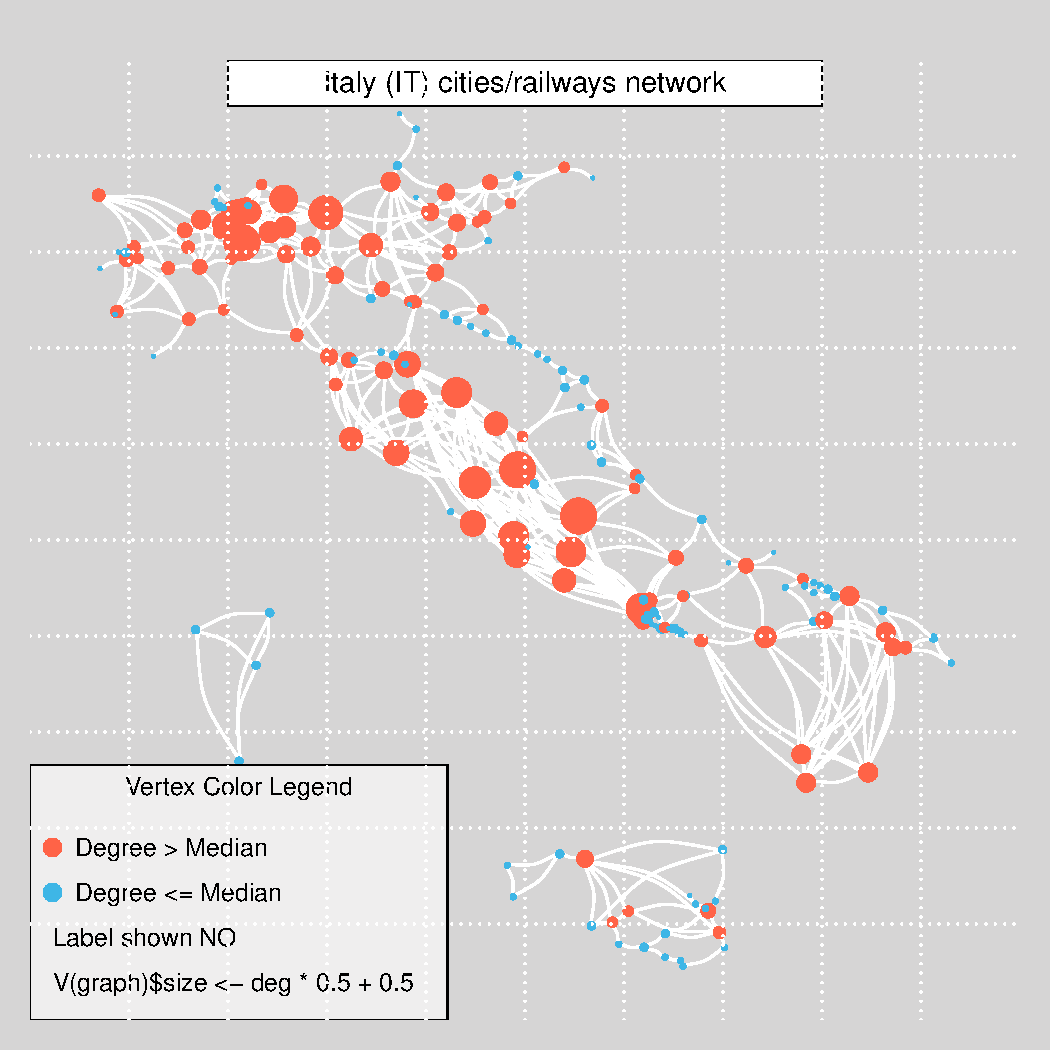
\includegraphics[width = 0.7\textwidth]{latex_source/images/railways/city_networks/IT_network.pdf}
\begin{subfigure}{}
    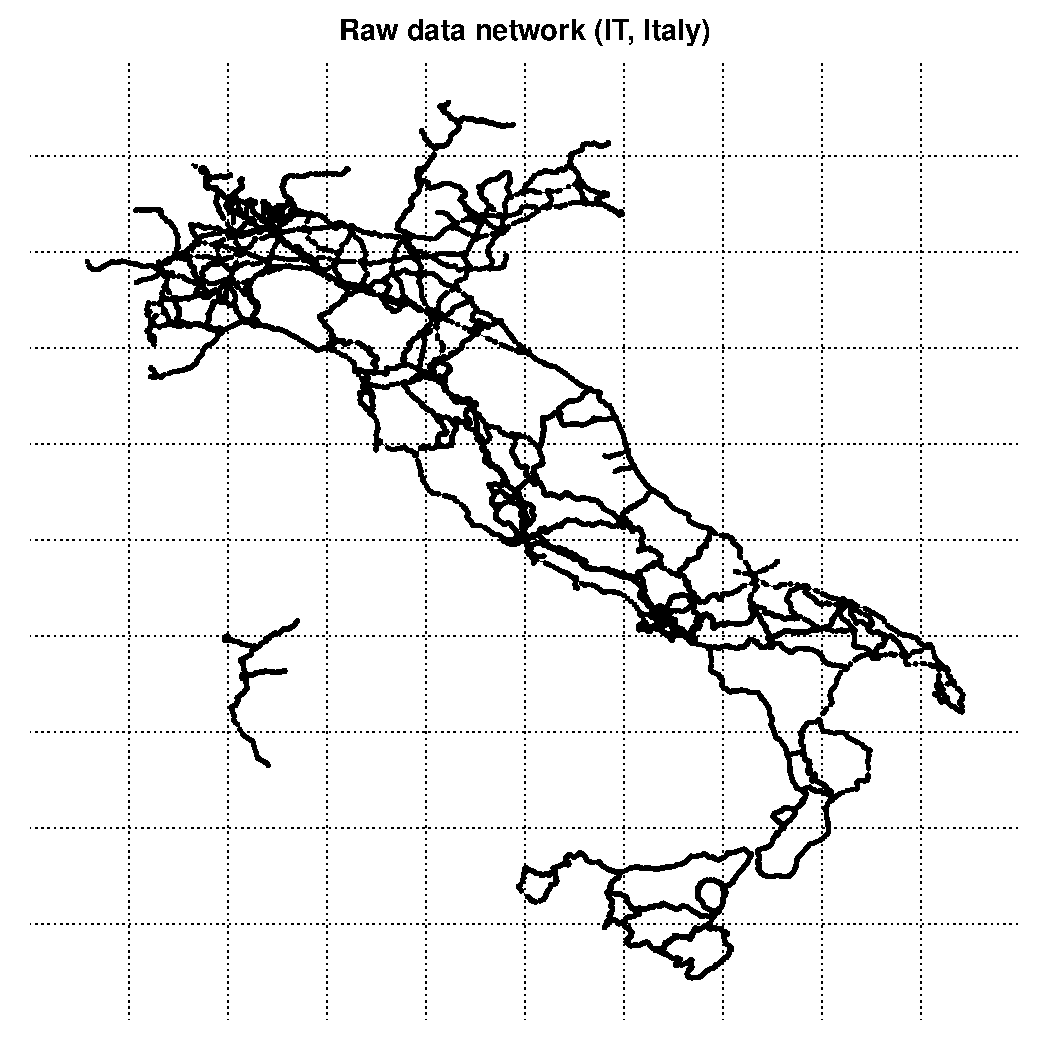
\includegraphics[width = 0.3\textwidth]{latex_source/images/railways/raw_networks/raw_IT_network.pdf}
\end{subfigure}
\begin{subfigure}{}
    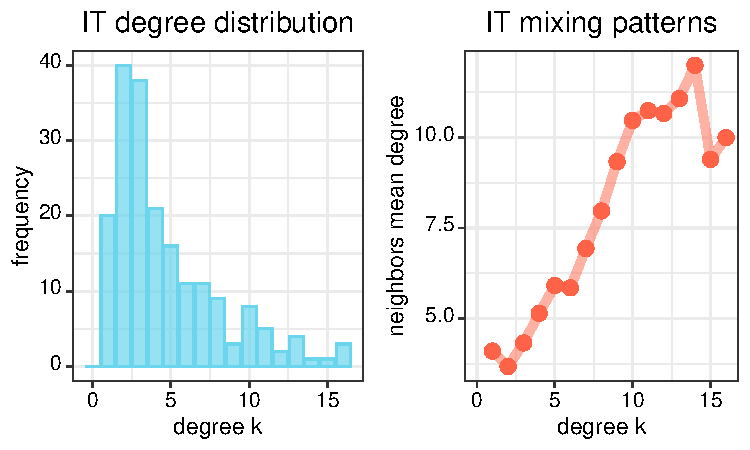
\includegraphics[width = 0.6\textwidth]{latex_source/images/railways/city_network_analysis/IT_analysis.pdf}
\end{subfigure}
\caption{IT (Italy) cities/ railways networks. Notice for instance the high density of edges in the center-left zone of the graph: it is a consequence of the fact that the stations "Roma Termini" and "Roma Tiburtina" are missing from file "RailrdC.shp" ! Many stations result directedly connected where in reality they are not because Rome stations are in between.}
\label{fig:rail_results}
\end{figure}
\newpage
\section*{Appendix}
\addcontentsline{toc}{section}{Appendix}
\subsection*{Supplementary figures}
\begin{figure}[H]
    \centering
    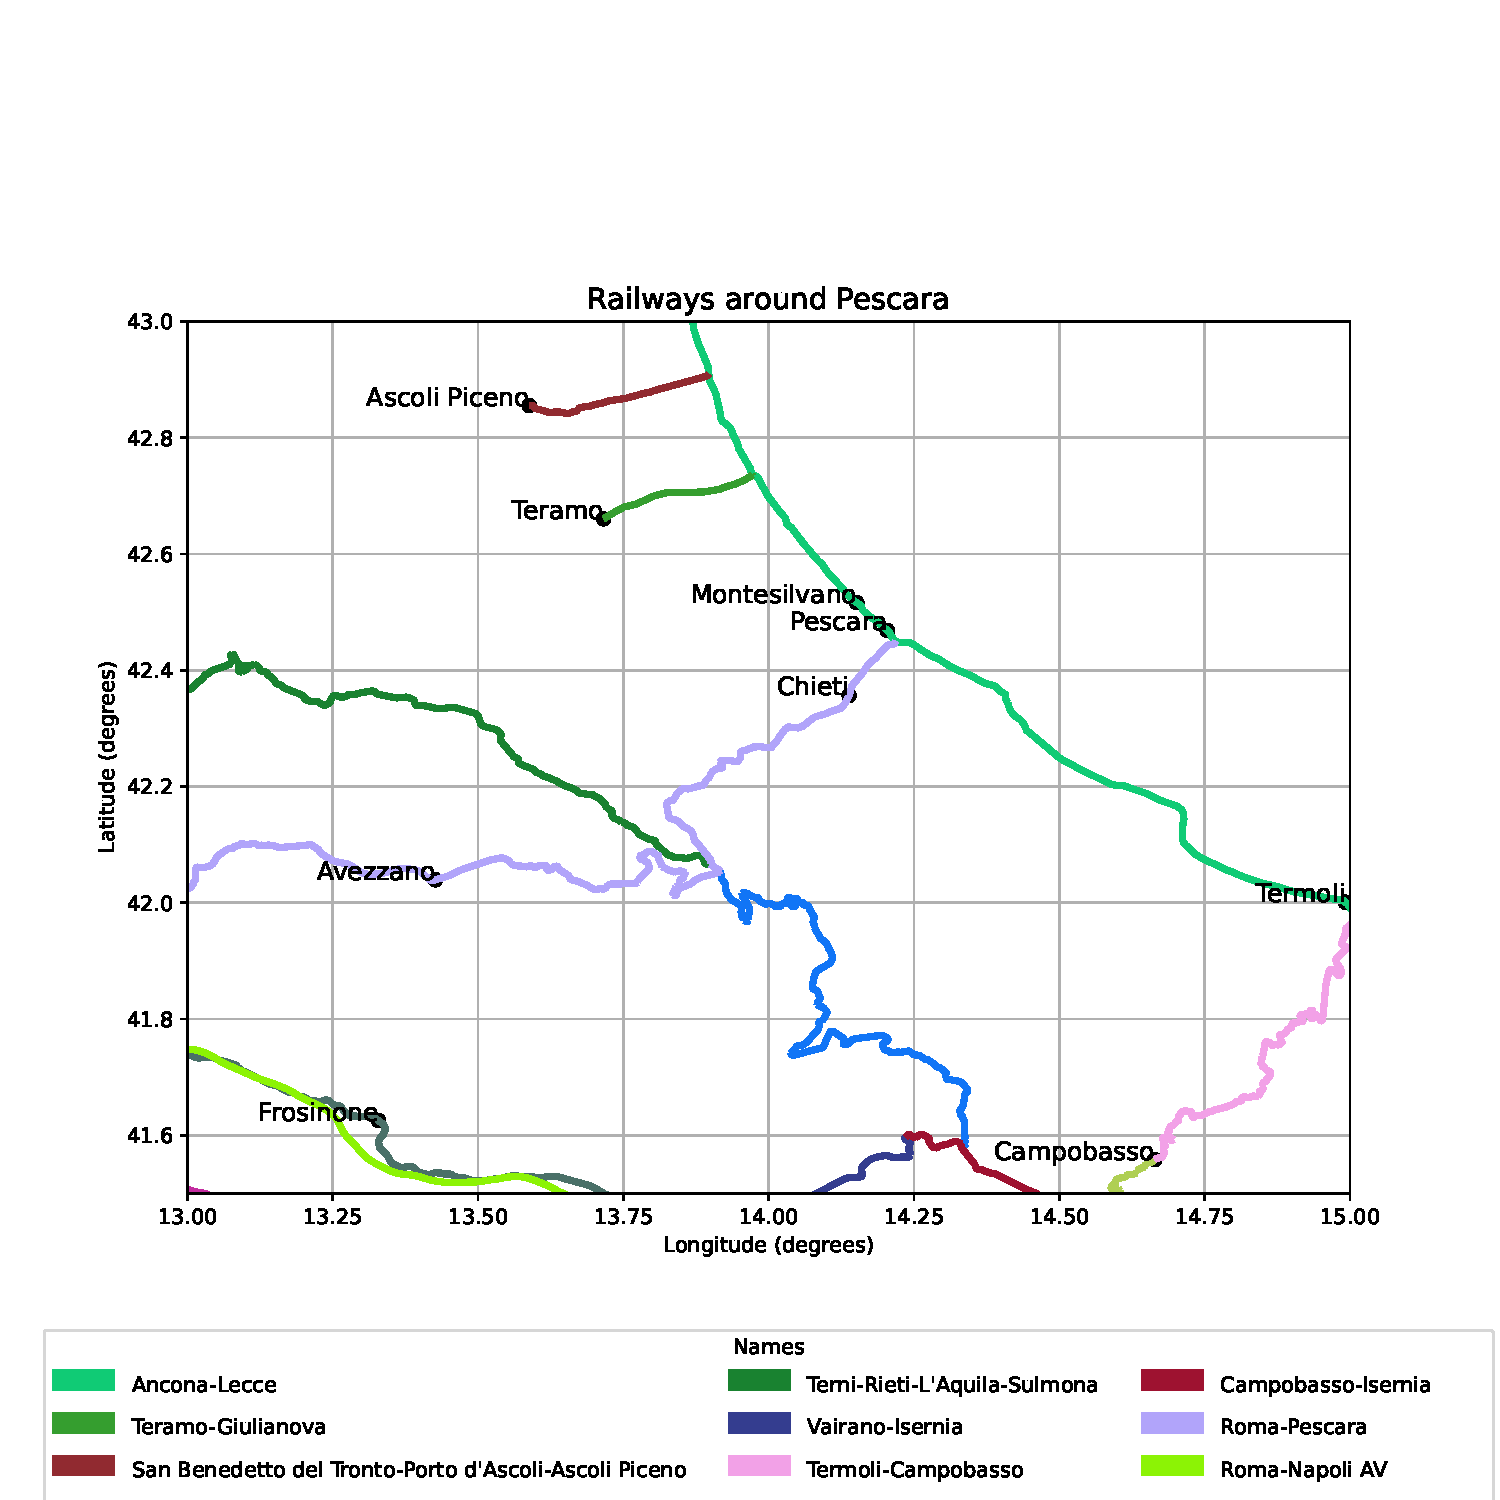
\includegraphics[width= \textwidth]{latex_source/images/railways/pescara_area.pdf}
    \caption{An example to justify the need for the "is near city" check: the rail bifurcation "Roma - Pescara" joins the "Ancora - Lecce" rail just before entering Pescara from south. Without the check implementation, edge "Termoli-Chieti" is created whereas in reality it does not exist: a train heading to Chieti must first stop in Pescara. }
    \label{fig:pescara_area}
\end{figure}






\chapter{Bibliography}
\begin{group}
\let\clearpage\relax
\phantomsection
\defbibheading{myheading}[My Bibliography]{%
  \section*{#1} % Puoi personalizzare il comando \section* per definire lo stile del titolo
}
\printbibliography[
keyword={turing},
heading=myheading,
title={Task 18: Turing Patterns}
]
\medskip
\newline
\noindent
\textbf{A note to the bibliography.}
This assignment specifically focuses on Turing patterns in \textit{networks}, with recommendation to replicate the findings presented in \cite{main_network}. However, for someone unfamiliar with Turing patterns, a few preliminary read may be necessary. Article \cite{bio_article}, targeted at biologists, offers an intuitive overview of the concept with minimal mathematical details. To delve deeper into the mathematical foundations, \cite[][\textit{Chapter 2: Spatial Pattern Formation with Reaction Diffusion Systems}]{murray} provides a comprehensive and detailed explanation of Turing Patterns in a continuous medium. Another valuable resource is \cite[][\textit{Chapter 7: The Turing Model for Biological Pattern Formation}]{altbook}, which, while shorter than Murray’s chapter, still offers insightful observations.   

\printbibliography[
keyword={ising},
heading=myheading,
title={Task 01: Ising Model}
]
\printbibliography[
keyword={voter},
heading=myheading,
title={Task 28: Voter Model}
]
\end{group}
\end{document}


